% !TEX root = ../main.tex

\glsresetall


\topquote[11cm]{
Two distinct elements are included under the term ``inheritance'' -- \\
the transmission, and the development of characters.
}{Charles Darwin, The Descent of Man}

%
\chapter{Introduction}
\label{ch:introduction}
\minitoc
%


-- mendel, pioneers in genetics, dna, genotyping, sequencing, data
-- one of the main goals: finding what causes disease, \eg for therapeutic application
-- insights and new challenges
-- objectives


focus of this thesis
to develop novel strategies and computationally tractable methods

GWAS has resulted in the successful identification of genetic factors implicated in heritable diseases
however, there are shortcomings and challenges
one shortcoming relates to not yet realised translation of findings into therapeutic application
a reason for this, for example is that GWAS do not yield the causal variant itself


In this thesis, I address the problems posed by rare genetic variants, and provide solutions to particular questions they raise.
These solutions take the form of new statistical models, methods, and computational algorithms, which I developed, first, in order to learn about particular properties of rare variants in the context of a specific analytical question, second, to demonstrate the viability of my methodology and, third, to enable application to large genetic datasets.

% It is a truth universally acknowledged that a student in possession of a good problem must be in want of a solution.\footnote{Modified from the first sentence of the novel \emph{Pride and Prejudice} by Jane Austen (1813), which is a story about learning from past events, gaining insights into errors, and overcoming problems; a theme that foreshadows the objectives of this thesis.}
% In this thesis, I address the problem of rare genetic variants, to which I raise particular questions, for which I provide the solutions.
% These solutions take the form of new statistical models, methods, and computational algorithms, which I developed, first, to learn about particular properties in context of the questions asked, second, to demonstrate the viability of my methodology and, third, to enable large-scale application to genetic datasets.
% Before I introduce the relevant questions, the following \n{2}~questions need to be resolved.

\paragraph{What are rare variants and why are they a problem?}
Recent advances in genotyping and sequencing technologies have enabled research on an unprecedented scale.
% but which has revealed some of the limits
% in our understanding
% of what can be inferred from genetic data using existing methods.
One major insight gained from the extensive study of the (human) genome is that most of the genetic variation between individuals sits at \emph{common} sites, but most variant sites are \emph{rare}.


\paragraph{...}


It is important to note that this thesis is less concerned with the discovery, for example, of previously unknown associations between (rare) variants and some complex disease or disorder, but much more so with the development of novel strategies that enable future discoveries.


; novel insights have been gained and deeper questions can now be asked.


%
% -- The size of available data has grown, posing new challenges to genetic analysis.
%
% -- One major interest: rare variants; due to their `novelty' (hypothetical before, now seen in abundance) and `challenge' (too low in frequency to determine effects, even in very large datasets).
%
% -- Brief background on rare variants: presumed young age, thereby mostly population specific, may be implicated in complex disease (anyway in Mendelian disease).
%
% -- There are several problems unsolved in regards to rare variants: not well enough captured in existing data due to population-specificity, existing methods are largely unable to make inference based on rare variants, likely to result in high error rare (e.g. imputation, phasing).
%
% -- Focus of this thesis: the development of novel statistical methods, first, to enable analysis on an even larger scale through integration of data, in particular for GWAS; second, to harness the information that is available directly through rare variants.
%
% -- Intuition: due to their presumed young age, rare variants are ideally suited to serve as anchor points to identify IBD; because young age implies long IBD tracts.
%
% -- Major insight gained: we have reached the point at which it is possible to estimate the age of a rare allele!
%
% -- Why this is useful: to gain insights into genetic architecture of traits, e.g. though correlation with phenotypic consequence; to record relations between age and frequency to reveal patterns of selection; to enable novel way of analysing genetic variation (e.g. at variants other than rare variants, if seen to be linked due to sitting on same IBD segment).
%
% -- Thus, this thesis is situated at the intersection between population genetics (for statistical inference) and medical genetics (for purpose).
%
% -- To begin with, the following sections provide a summary and definition of relevant topics.


% 	Genetic and environmental factors are key forces in shaping an individual’s predis- position to disease. Ultimately the hope is that we will be able to translate insights from the genetic makeup of diseases to therapies and cures. In the past two decades significant strides have been made in understanding the genetic makeup of complex traits.




%
\section{Basic concepts and terminology}
%

This section outlines the biological concepts relevant to define basic terminology as used in this thesis.

%All known living organisms are composed of \n{1} or up to several billion cells, most of which contain a complete copy of the genome of the individual organism.
The term \emph{genome}, which was coined almost a century ago \citep{Winkler1920}, refers to the totality of the genetic hereditary information and its organisation into \emph{chromosomes}.
The number of chromosomes is characteristic for an organism, as is the number of chromosome sets, referred to as \emph{ploidy}.
Cells with only \n{1} chromosome, or \n{1} set of chromosomes, are said to be \emph{haploid}; for example, bacterial cells contain a single chromosome, as do mitochondria in animal cells or chloroplasts in the cells of plants and algae.
In most animal species, such as humans, somatic cells typically carry \n{2} sets of chromosomes, where \n{1} set is derived from each parent; \ie they are said to be \emph{diploid}.
%Organisms with more than \n{2} sets are \emph{polyploid}, which is seen in some plant species, but less commonly among animal species.
In sexually reproducing organisms, chromosomes can be further distinguished into \emph{autosomes} and \emph{allosomes} (or ``sex~chromosomes'').
For example, human cells carry \n{22}~autosome pairs, which are \emph{homologous} in both males and females, and \n{1} set of allosomes (X~and~Y~chromosomes), which determine sex and thus differ in males and females.

\Gls{dna} forms the molecular basis of what is commonly referred to as ``genetic~material''.
The molecular structure of \gls{dna} was first described by \citet{Watson:1953ug} on basis of X-ray diffraction data by Rosalind~Franklin.
A chromosome is a single \gls{dna} molecule composed of \n{2} strands that form a double helical structure.
Each strand is a chain of \emph{nucleotide} subunits containing \n{1} of \n{4} \emph{nucleobases}; adenine~(\texttt{A}), guanine~(\texttt{G}), cytosine~(\texttt{C}), and thymine~(\texttt{T}), which constitute the alphabet of the genetic code.
The DNA~double~helix is held together through hydrogen bonds between complementary nucleobases on opposite strands, where \texttt{A} can only pair with \texttt{T} and \texttt{C} only with \texttt{G}.
% \emph{purine} bases (A~or~G) can only pair with \emph{pyrimidine} bases (C~or~T).
The human genome, for example, contains more than 3~billion such \emph{base~pairs}.
The chemical structure of the DNA~double~helix is illustrated in \cpref{fig:info_dna}.

%
%!TEX root = ../../main.tex


\begin{figure}[!htb]

\makeatletter
\newcommand*\derivesubmol[4]{%
    \saveexpandmode\saveexploremode\expandarg\exploregroups
    \csname @\ifcat\relax\noexpand#2first\else second\fi oftwo\endcsname
        {\expandafter\StrSubstitute\@car#2\@nil}
        {\expandafter\StrSubstitute\csname CF@@#2\endcsname}
    {\@empty#3}{\@empty#4}[\temp@]%
    \csname @\ifcat\relax\noexpand#1first\else second\fi oftwo\endcsname
        {\expandafter\let\@car#1\@nil}
        {\expandafter\let\csname CF@@#1\endcsname}\temp@
    \restoreexpandmode\restoreexploremode
}
\makeatother

\renewcommand*\printatom[1]{\ensuremath{\mathsf{#1}}}

\setatomsep{2.5em}
\setcrambond{1ex}{1pt}{2pt}

\definesubmol{rt1}{-[2]rt1}
\definesubmol{rt2}{-[6,.6]rt2}

\definesubmol{ribose}{%
	-[::-90,1.5]%
	    (%
	        -[::115,1.35]O%
	        -[::-50,1.35]%
	    )%
	<[::45,1]%
	    (%
	      -[::45,,,,line width=3pt,shorten <=-.5pt,shorten >=-.5pt]%
	          (!{rt2})%
	      >[::45,1]%
	          (!{rt1})%
	     )%
}

\definesubmol{OH_group}{-[::-45,1.2]OH}

\definesubmol{phosphate}{%
	-[::-45,1.2]O%
	-[::0,1.5]P%
	(%
		-[::-90,1.5]O{^-}%
	)%
	(%
		=[::0,1]O%
	)%
	-[::90,1.5]O%
}

\definesubmol{phosphate_lhs_beg}{%
	O{^-}%
	-[::-90,1.5]P%
	(%
		=[::0,1]O%
	)%
	(%
		-[::-90,1.5]O{^-}%
	)%
	-[::90,1.5]O%
}

\definesubmol{phosphate_rhs_beg}{%
	O{^-}%
	-[::90,1.5]P%
	(%
		-[::-90,1.5]O{^-}%
	)%
	(%
		=[::0,1]O%
	)%
	-[::90,1.5]O%
}

\definesubmol{adenine}{%
	N*5%
	(%
		[:72]-*6%
		(%
			-N=-N%
			(%
				-[:15,2.3,,,dash pattern=on 1pt off 1pt]%
			)%
			=(%
			-NH_2%
			-[:16,2.2,,,dash pattern=on 1pt off 1pt]%
			)-%
		)=-N=-%
	)%
}
\definesubmol{adenineR}{%
	N*5%
	([:138]-=N-*6%
	(-(-[,,,2]H_2N%
	)=N(%
	)-=N-)=-)%
}

\definesubmol{guanine}{%
	N*5%
	(%
		[:72]-*6%
		(%
			-N=%
			(%
				-NH_2%
				(-[:16,2.2,,,dash pattern=on 1pt off 1pt])%
			)%
			-NH%
			(-[:15,2.4,,,dash pattern=on 1pt off 1pt])-%
			(%
			=O(-[:16,2.1,,,dash pattern=on 1pt off 1pt])%
			)-%
		)%
		=-N=-%
	)%
}

\definesubmol{guanineR}{%
	N*5%
	(%
		[:138]-=N-*6%
		(-%
			(%
				=O%
			)%
				-[,,,2]HN-%
			(%
				-[,,,2]H_2N%
			)%
			=N-%
		)%
		=-%
	)%
}

\definesubmol{cytosine}{%
	N*6%
	([:60]-%
		(%
			=O%
			(-[:22,2.05,,,dash pattern=on 1pt off 1pt])%
		)%
		-N%
		(-[:20,2.3,,,dash pattern=on 1pt off 1pt])%
		=%
		(%
			-NH_2%
			(-[:22,2.2,,,dash pattern=on 1pt off 1pt])%
		)%
		-=-%
	)%
}
\definesubmol{cytosineR}{%
	N*6([:150]-=-(-[,,,2]H_2N%
	)=N-%
	(=O)-)%
}

\definesubmol{thymine}{%
	N*6%
	([:60]-%
		(%
			=O%
		)%
		-NH%
		(%
			(-[:22,2.3,,,dash pattern=on 1pt off 1pt])%
		)-%
		(%
			=O%
			(-[:22,2.1,,,dash pattern=on 1pt off 1pt])%
		)-%
		(-)%
		=-%
	)%
}
\definesubmol{thymineR}{%
	N*6([:150]-=(-)-%
	(=O)%
	-[,,,2]HN%
	-(=O)-)%
}

\derivesubmol{deoxyribose}{ribose}{(!{rt2})}{}

\derivesubmol{A_group_lhs}{deoxyribose}{!{rt1}}{-[::-45,1.5]!{adenine}}
\derivesubmol{G_group_lhs}{deoxyribose}{!{rt1}}{-[::-45,1.5]!{guanine}}
\derivesubmol{C_group_lhs}{deoxyribose}{!{rt1}}{-[::-45,1.5]!{cytosine}}
\derivesubmol{T_troup_lhs}{deoxyribose}{!{rt1}}{-[::-45,1.5]!{thymine}}

\derivesubmol{A_group_rhs}{deoxyribose}{!{rt1}}{-[::-45,1.5]!{adenineR}}
\derivesubmol{G_group_rhs}{deoxyribose}{!{rt1}}{-[::-45,1.5]!{guanineR}}
\derivesubmol{C_group_rhs}{deoxyribose}{!{rt1}}{-[::-45,1.5]!{cytosineR}}
\derivesubmol{T_group_rhs}{deoxyribose}{!{rt1}}{-[::-45,1.5]!{thymineR}}


\centering
%\hrulefill \\
%\vspace{5pt}


\tikzset{
    ncbar angle/.initial=90,
    ncbar/.style={
        to path=(\tikztostart)
        -- ($(\tikztostart)!#1!\pgfkeysvalueof{/tikz/ncbar angle}:(\tikztotarget)$)
        -- ($(\tikztotarget)!($(\tikztostart)!#1!\pgfkeysvalueof{/tikz/ncbar angle}:(\tikztotarget)$)!\pgfkeysvalueof{/tikz/ncbar angle}:(\tikztostart)$)
        -- (\tikztotarget)
    },
    ncbar/.default=0.25cm,
}
\tikzset{Lbrace/.style={ncbar=-0.25cm}}
\tikzset{Rbrace/.style={ncbar=0.25cm}}

\scalebox{0.9}{%
\begin{tikzpicture}[txt/.style={font=\sffamily\slshape\bfseries\scriptsize,text=gray!60,text width=2.5cm}]
\tiny

% \filldraw[even odd rule,draw=white,inner color=red!40,outer color=white] (0.5,6.95) circle (0.5);
% \filldraw[even odd rule,draw=white,inner color=red!40,outer color=white] (-0.35,6.95) circle (0.4);
% \filldraw[even odd rule,draw=white,inner color=green!50,outer color=white] (0.95,4.4) circle (0.5);
% \filldraw[even odd rule,draw=white,inner color=yellow!80,outer color=white] (2.15,1.8) circle (0.5);
% \filldraw[even odd rule,draw=white,inner color=blue!25,outer color=white] (4,-0.78) circle (0.5);
% \filldraw[even odd rule,draw=white,inner color=blue!25,outer color=white] (3.15,-0.78) circle (0.4);
%
% \filldraw[even odd rule,draw=white,inner color=yellow!80,outer color=white] (2.875,7.8) circle (0.5);
% \filldraw[even odd rule,draw=white,inner color=blue!25,outer color=white] (3.45,4.855) circle (0.5);
% \filldraw[even odd rule,draw=white,inner color=blue!25,outer color=white] (4.2,5.255) circle (0.4);
% \filldraw[even odd rule,draw=white,inner color=red!40,outer color=white] (4.65,2.25) circle (0.5);
% \filldraw[even odd rule,draw=white,inner color=red!40,outer color=white] (5.35,2.65) circle (0.4);
% \filldraw[even odd rule,draw=white,inner color=green!50,outer color=white] (6.35,0.05) circle (0.5);

\node[draw=white] (UL) at (-5,9.5) {};
\node[draw=white] (UR) at (11,9.5) {};
\node[draw=white] (LL) at (-5,-3) {};
\node[draw=white] (LR) at (11,-3) {};

\draw [draw=gray!40,ultra thick] (-0.75,8.25) to [Lbrace] (-0.75,5.85);
\draw [draw=gray!40,ultra thick] (0.4,5.5) to [Lbrace] (0.4,3.1);
\draw [draw=gray!40,ultra thick] (1.5,2.85) to [Lbrace] (1.5,0.55);
\draw [draw=gray!40,ultra thick] (2.75,0.4) to [Lbrace] (2.75,-1.95);

\node[txt] at (0.36,6.05) {Adenine};
\node[txt] at (1.5,3.3) {Cytosine};
\node[txt] at (2.6,0.725) {Thymine};
\node[txt] at (3.85,-1.76) {Guanine};

\draw [draw=gray!40,ultra thick] (3.625,8.9) to [Rbrace] (3.625,6.25);
\draw [draw=gray!40,ultra thick] (4.75,6) to [Rbrace] (4.75,3.8);
\draw [draw=gray!40,ultra thick] (5.9,3.5) to [Rbrace] (5.9,1.275);
\draw [draw=gray!40,ultra thick] (7.1,0.9) to [Rbrace] (7.1,-1.55);

\node[txt] at (3.95,6.4) {Thymine};
\node[txt] at (5.11,3.99) {Guanine};
\node[txt] at (6.27,1.445) {Adenine};
\node[txt] at (7.41,-1.4) {Cytosine};

\node[txt] at (-2.65,8.55) {5' end};
\node[txt] at (6,9) {3' end};
\node[txt] at (2.1,-2.65) {3' end};
\node[txt] at (10.65,-2.2) {5' end};

\node at (1,3) {%
\chemfig{%
  !{phosphate_lhs_beg}%
	!{A_group_lhs}!{phosphate}%
	!{C_group_lhs}!{phosphate}%
	!{T_troup_lhs}!{phosphate}%
	!{G_group_lhs}!{OH_group}%
}};%
\node at (6.25,3.5) {%
\chemfig{%
  !{phosphate_rhs_beg}%
	!{C_group_rhs}!{phosphate}%
	!{A_group_rhs}!{phosphate}%
	!{G_group_rhs}!{phosphate}%
	!{T_group_rhs}!{OH_group}%
}};
\end{tikzpicture}%
}

\Caption{The chemical structure of DNA}
{
The \gls{dna} molecule is a long chain polymer of individual nucleotide building blocks.
Each nucleotide is composed of a phosphate residue, a deoxyribose sugar (pentose), and a nucleobase (adenine, guanine, cytosine, or thymine).
The phospho-deoxyribose subunits are identical at each nucleotide and form the backbone of a \gls{dna} strand along which the sequence of nucleobases may vary.
The \gls{dna} in living cells is typically composed of \n{2} complementary strands, which are connected through hydrogen bonds between complementary nucleobases.
The figure shows a hypothetical sequence of \n{4} base pairs, where hydrogen bonds (\emph{dotted} lines) can only be formed between nucleobases as indicated.
\Delete{This figure was generated in \LaTeX.}}
{fig:info_dna}
% \vspace{-5pt}
% \hrulefill%
\end{figure}

%

It is the sequence of base~pairs along a chromosome which stores and thereby constitutes ``genetic~information''.
The expression of information typically occurs at a \emph{gene} coding region of a chromosome.
A gene is an organised structure of \gls{dna} elements, which can be distinguished into regulatory sequence regions and protein-coding regions (\emph{exons}) that can be separated by non-coding \gls{dna} segments (\emph{introns}).
% Genes are typically
% gene product, \eg a protein.
The genetic code assigns a specific amino~acid to a triplet of \n{3} consecutive nucleobases, which is referred to as a \emph{codon}.
The directional order of codons instructs the \emph{transcription} from double-stranded \gls{dna} into single-stranded \gls{rna} and, from \gls{rna}, the \emph{translation} into proteins.
Gene expression thereby determines and regulates cell growth and maintenance, as well as the development of an organism and its ability to interact with and react to the environment.

The sum of such observable characteristics is referred to as the \emph{phenotype} of an individual.
The expression of phenotypic traits varies among the members of a population due to genetic variation as well as environmental influences.
For example, traits such as blood type or eye colour are determined genetically, whereas most of the phenotypic variability seen in a population arises from interactions between genetic and environmental factors.
Typical examples are the effects of diet or stress on complex traits such as body weight or health.

% The phenotype of an individual may affect both its physical fitness as well as its fitness in an evolutionary sense.
% In population genetics, the term \emph{fitness} is a measure of the adaptation of an individual to its environment.
% The adaptive value of an individual's phenotype (or rather the sum of genetic factors influencing its phenotype) is measured according to how it affects the number of the individual's offspring.
% The phenotypic (and thereby genetic) disposition of an individual is said to increase its fitness if it produces a higher number of offspring relative to other individuals of the population.
% This is because its ``genes'' have a higher chance to survive within the population over the course of generations.
% Fitness
% selection, which can be distinguished into \emph{natural selection} if determined by the environment, or \emph{sexual selection} if the phenotypic traits of an individual affect its reproductive success.
% The driving force behind


Note that the meaning of the word \emph{gene} has changed over time \citep[\eg see][]{slack2014genes}.
Historically, that is before the molecular basis of genetic inheritance was discovered, a gene was informally defined as the smallest unit of heredity, referring to the physical determinant of a characteristic that is transmitted from parent to offspring.
This definition is convenient to mathematically describe the process of genetic inheritance and shall therefore be used in the remainder of this thesis.
Further, a \emph{locus} (plural~\emph{loci}) refers to the physical location of a gene on a chromosome, but may also be used in reference to the position of a single nucleotide (or \emph{site}) in the genome.
A gene may be observed in different variant forms in the population,
where a particular form is distinguished as an \emph{allele}.
If a set of sites on a single chromosome is considered, \ie the alleles observed at different loci, the term \emph{haplotype} is used.
A haplotype thus denotes a vector of observed alleles at \n{1} or multiple sites on a chromosome; \eg the haplotype at a single site refers to the allelic state observed at that locus.
In contrast, the term \emph{genotype} refers to the sum of the inherited genetic information at \n{1} or multiple sites.
While \n{1} \emph{maternal} and \n{1} \emph{paternal} haplotype can be distinguished, the genotype at a single locus denotes the sum of alleles inherited from both parents (also referred to as ``allele dosage'').
An individual can be \emph{homozygous} for a particular allele at a given site if the allele is identical in both parents, or \emph{heterozygous} if the inherited alleles differ.

%
%!TEX root = ../../main.tex


\begin{figure}[!htb]
\centering
%\hrulefill \\
%\vspace{5pt}
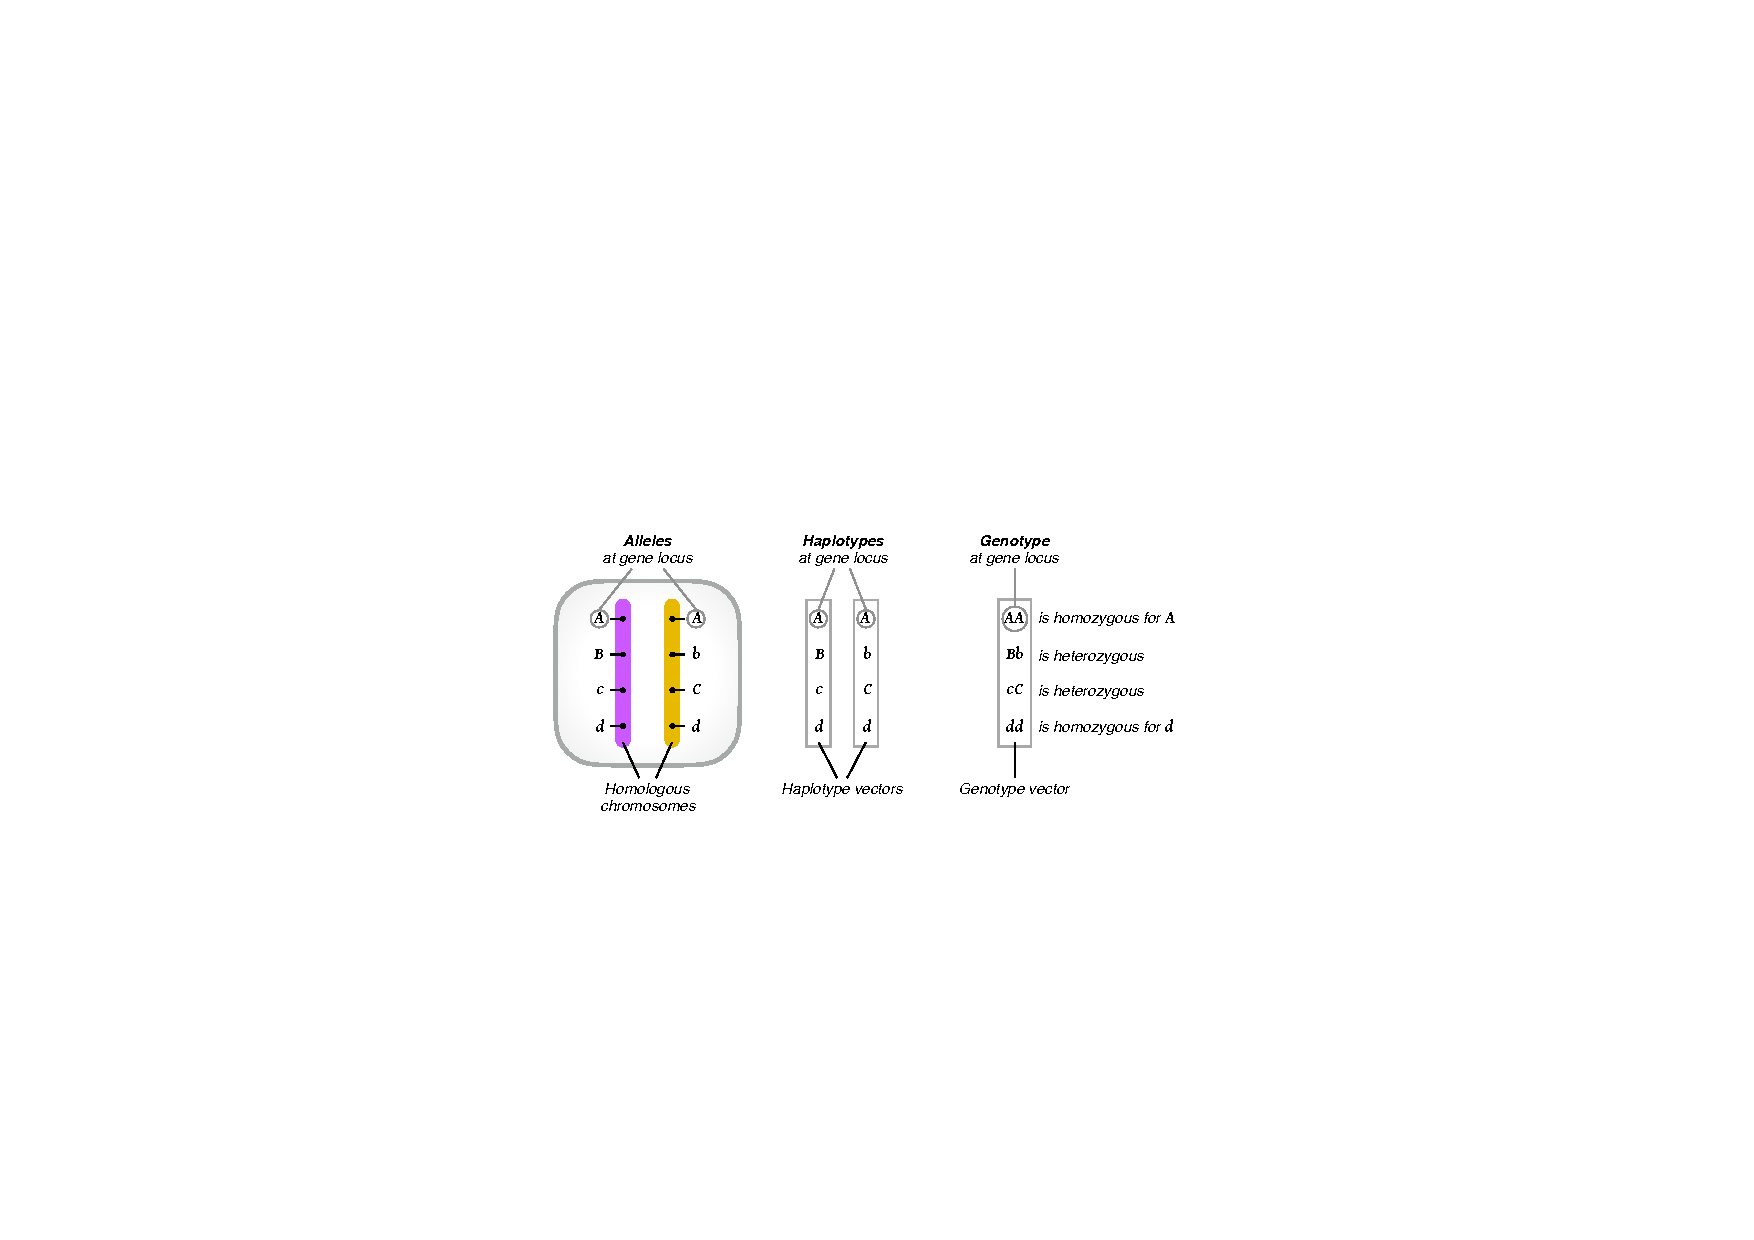
\includegraphics[width=0.8\textwidth]{./img/ch1/info_types}
\Caption{Alleles, haplotypes, and genotypes}
{A pair of homologous chromosomes is shown (\emph{left}) on which \n{4} gene loci are highlighted; labelled as $A$, $B$, $C$, and $D$.
Maternal and paternal chromosomes are shown in \emph{purple} and \emph{yellow} (arbitrarily coloured).
Each gene may have \n{2} allelic states (in this example), distinguished by capitalisation of the label.
Each chromosome has a corresponding haplotype at each locus (\emph{middle}).
Genotypes do not distinguish chromosomes and are represented as the sum of allelic information inherited from both parents (\emph{right}).
Note that the term \emph{haplotype} may refer to the allelic state observed at a single nucleotide or a set of alleles observed along a chromosome.
Likewise, the term \emph{genotype} may refer to the allelic dosage at a single site or a vector of observed genotypic information.}
{fig:info_types}
% \vspace{-5pt}
% \hrulefill%
\end{figure}

%

The terminology introduced in the last paragraph will be used throughout this thesis and is therefore further clarified in \cpref{fig:info_types}.
The following sections describe the main processes which generate genetic variation and, thereby, phenotypic variation in a population; namely mutation (\cref{sec:mutation}) and recombination (\cref{sec:recombination}).


%
\subsection{Mutation}
\label{sec:mutation}
%

A mutation constitutes a lasting change in the genetic sequence.
The change may initially be only present in \n{1} cell, but it is passed on to daughter cells in the course of successive cell divisions (\emph{mitosis}).
If mutations occur in the germline, \ie germ cells which give rise to haploid \emph{gametes} (sperm and egg cells) during \emph{meiosis}, the nucleotide sequence is permanently altered in all cells of the progeny.
If a mutation has no effect on the reproductive success of an individual, it is said to be selectively \emph{neutral}; otherwise, a mutation may lead to a selective advantage or disadvantage, \eg due to a \emph{beneficial} or \emph{deleterious} effect on the phenotype, respectively.
In humans, the average rate of mutation per site and per generation, denoted by $\mu$, is typically as low as \n{1} mutation event every 100~million base~pairs.
More specifically, recent studies suggest a mutation rate of ${\mu\approx\num{1.1e-8}}$ \citep{Roach:2010ef} or ${\mu\approx\num{1.2e-8}}$ \citep{Scally:2012fe}.
%Mutations that are found only in the genome of the offspring but in neither of the parents are referred to as \emph{de~novo} mutations.

A mutation event may occur due to imperfect \gls{dna} replication during cell division or due to errors in the \gls{dna} repair process.
A change at a single position on the chromosome results from a \emph{substitution} of \n{1} base for another, which in sample data is observed as a \gls{snp}.
Also, nucleotides may be added to or removed from the sequence, due to \emph{insertions} or \emph{deletions} respectively, which are commonly referred to as \emph{indels}.
%Dependent on the number and position of inserted or deleted nucleotides, gene expression may be altered or hindered due to a codon offset during transcription, which is referred to as a \emph{frameshift} mutation.
Larger changes to the chromosomal structure may also be distinguished.
However, this thesis is mainly concerned with genetic variation observed at individual positions in the genome.
In the following, the term ``mutation'' is used in reference to substitutions at single loci that result in observable \glspl{snp} in sample data.

Most mutations seen in genomic datasets are \emph{biallelic}, meaning that there are not more than \n{2} gene versions observed in a sample.
However, multiple allelic types may exists in a population.
In the general case, biallelic \glspl{snp} are assumed.

%Due to the ``degeneracy'' of the genetic code, different codons may encode the same amino acid such that a substitution of one base may not alter the amino acid sequence in the protein product.

%Others may lead to a \gls{lof} of the gene product, whereas only few may lead to a \gls{gof} and, thereby, to the possibility of selective advantage.


%
\subsection{Recombination}
\label{sec:recombination}
%

% Sexually reproducing organisms are generally thought of to have an evolutionary advantage over
% and are therefore thought of having an evolutionary advantage over non-sexual species \citep{Otto:2002cn}.

%Both mutation and recombination shape the genetic variability in a population.

Recombination refers to the reorganization of alleles during meiosis in sexually reproducing organisms, which is facilitated through the physical exchange of genetic material between maternal and paternal chromosomes, such that new combinations of alleles are generated and transmitted to the offspring.
% Both the random distribution of homologous chromosomes during meiosis, as well as the process of recombination contribute to the genetic variability in the population.
%contributes to the formation of gametes.
For example, consider the haplotypes at \n{2} loci in an individual which is heterozygous for both the alleles at these loci.
Given gene~$\mathcal{A}$ with alleles $A$~and~$a$, and gene~$\mathcal{B}$ with alleles $B$~and~$b$, the observed allelic configurations are $(A,B)$ on \n{1} of the chromosomes and $(a,b)$ on the other.
If no recombination occurs between the \n{2} loci during meiosis, the resulting gametes retain the configuration as present in the parental chromosomes; \ie the offspring may either receive $(A,B)$ or $(a,b)$.
In presence of recombination, in particular if the number of recombination events between both loci is odd, the association between the \n{2} loci is broken such that either $(A,b)$ or $(a,B)$ are transmitted to the offspring.
% Note that the genotypes at these \n{2} do not change, because genotype~$Aa$ cannot be distinguished from genotype~$aA$.
An even number of recombination events reverts the configuration of alleles at the \n{2} focal positions, such that recombination cannot be inferred from variation observed at those loci.
Both cases (odd and even numbers of recombination events) are illustrated in \cpref{fig:info_meiosis}.
For simplicity, the figure shows only \n{1} pair of homologous chromosomes on which the alleles of genes $\mathcal{A}$ and $\mathcal{B}$ are indicated.

%
%!TEX root = ../../main.tex


\begin{figure}[!htb]
\centering
%\hrulefill \\
%\vspace{5pt}
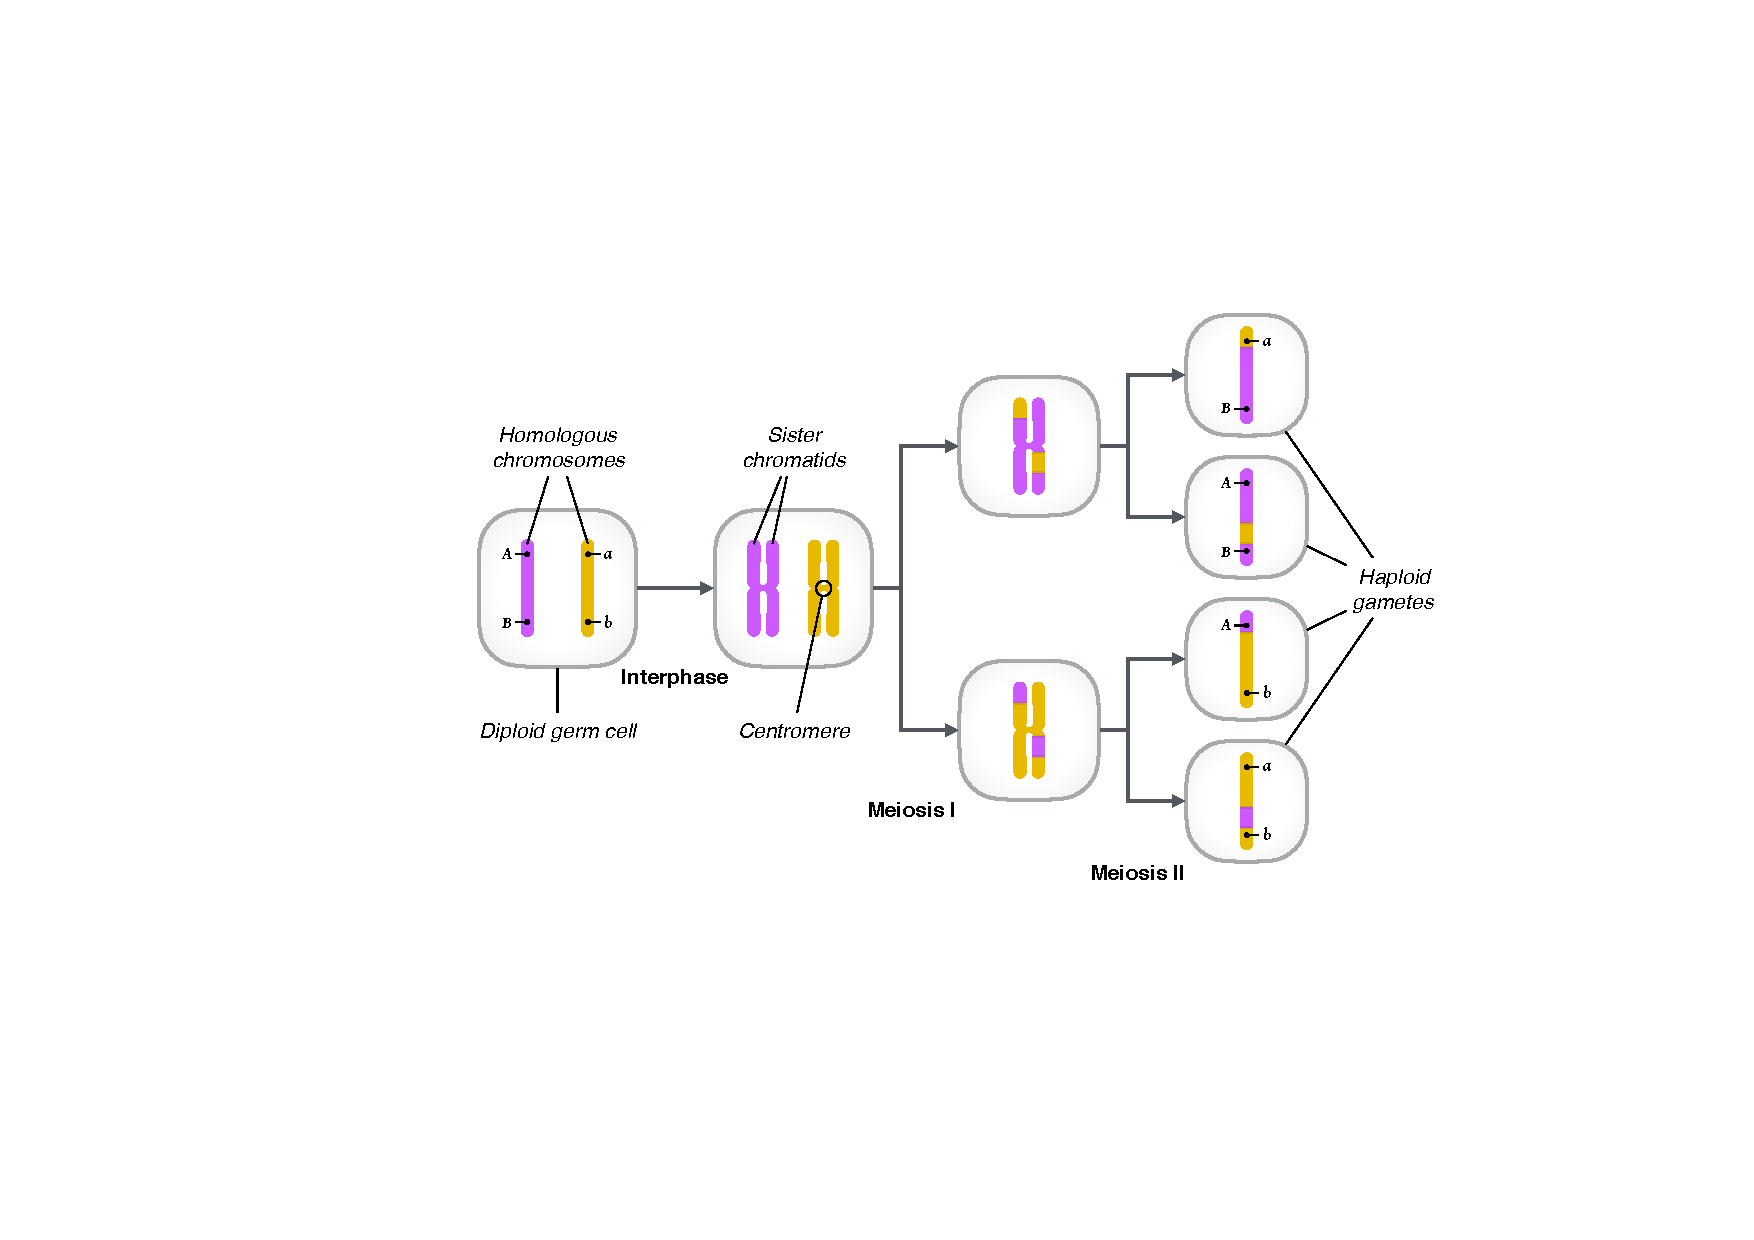
\includegraphics[width=0.9\textwidth]{./img/ch1/info_meiosis}
\Caption{Illustration of recombination during meiosis}
{\N{1} pair of homologous chromosomes is shown at the beginning of the meiotic cell cycle (\emph{left}).
Maternal and paternal chromosomes are shown in \emph{purple} and \emph{yellow} (arbitrarily coloured).
The allelic configuration at \n{2} sites is indicated on both chromosomes; $(A,B)$ and $(a,b)$.
\Gls{dna} sequences are replicated during the \emph{Interphase} of meiosis, where each chromosome forms \n{2} identical \emph{sister chromatids} which are held together at the \emph{centromere}.
Homologous chromosomes are paired at the beginning of the first cell division (\emph{Meiosis~I}), during which sequence segments are exchanged between chromatids through crossover.
In the second cell division (\emph{Meiosis~II}), the \n{4} chromatids are then separated into haploid gametes (\emph{right}).}
{fig:info_meiosis}
% \vspace{-5pt}
% \hrulefill%
\end{figure}

%

The meiotic cell cycle undergoes \n{2} cell divisions, \emph{Meiosis~I} and \emph{Meiosis~II}, such that \n{4} haploid gametes are produced from \n{1} diploid germ cell.
Prior to the first division, the \gls{dna} of all chromosomes is replicated during the \emph{Interphase} of meiosis.
Each of the replicated chromosomes thereby forms \n{2}~\emph{sister chromatids}, which are held together at a central region called the \emph{centromere}.
Recombination occurs during Meiosis~I along the homologous regions of maternally and paternally derived chromatids.
\N{2} main mechanisms of recombination can be distinguished.
\begin{itemize}[leftmargin=1em]
	\item \textbf{Chromosomal crossover} refers to the overlap of \n{2} chromatids with subsequent, mutual exchange of homologous \gls{dna} segments.
	The exchange is initiated through a double-strand break in \n{1} of the chromatids, followed by a so called ``strand invasion'' on the opposite chromatid which leads to an equal cross-strand exchange.
	% The example of recombination between genes $\mathcal{A}$ and $\mathcal{B}$ given in the previous paragraph is a consequence of crossover.
	\item \textbf{Gene conversion} is a non-reciprocal exchange of genetic material.
	The \gls{dna} sequence at a section in \n{1} of the chromatids is replaced by a copy of the sequence on the opposite chromatid, resulting in the loss of its original sequence.
\end{itemize}
In a general context, chromosomal crossover is implied as the acting mechanism of recombination, whereas gene conversion is usually asserted specifically.

A direct consequence of meiotic recombination is the phenomenon of genetic \emph{linkage}, which was discovered by \citet{morgan1911} in experiments on  \textsl{Drosophila}.
Linkage describes the concept that genetic markers located in close proximity to each other are less likely to be separated by recombination during meiosis.
The frequency of recombination between \n{2} loci is therefore assumed to be proportional to their distance on a chromosome.
For example, a pair of markers is said to be \emph{linked} if they retain a significant statistical association to each other in a sample of individuals over the course of many generations.
Markers on different chromosomes are by default \emph{unlinked} due to the random distribution of homologous chromosomes during meiosis.
This idea was further developed by \citet{sturtevant1913}, who proposed that the probability of \n{2} markers being separated by crossover events can be used as a measure of the \emph{genetic distance}.
It was this idea that paved the way for the development of molecular and statistical methods for the purpose of \emph{linkage mapping} (or ``gene mapping''), through which it became possible, for example, to identify the physical location of particular genetic factors implicated in human disease.

By convention, the unit of genetic distance is called a \emph{Morgan}.
However, it is more common to express genetic distance in units of \gls{cM}, where ${1~\text{Morgan}}$ is equal to ${100~\text{cM}}$.
For example, if \n{2} loci sit 1~\gls{cM} apart on a chromosome, the expected number of crossover events between them is $0.01$ per generation, meaning that the \n{2} loci are separated once every \n{100} meioses on average.
In humans, a distance of 1~\gls{cM} corresponds to about 1~million base pairs; \ie 1~\gls{Mb}.
Since the genetic distance translates into the rate of recombination, denoted by $\rho$, the human genome exhibits an average rate of ${\rho \approx \num{1e-08}}$ per site per generation.
However, the recombination rate varies among chromosomes and more so along the length of each chromosome.

% revealed recombination hotspots


%
\section{Medical genetics}
%

%
\subsection{Mendelian disorder}
%

%
\subsection{Complex disease}
%


%
\section{Population genetics}
%

Over the last century, the field of population genetics has evolved from a mainly theoretical area of study into a more applied area of research.
More recently, the field has adapted to the exponential growth of available molecular data and continues to fill a niche in the computational sciences so as to be able to analyse the increasing amounts of data and to answer questions of biological as well as medical meaning.
This section outlines the statistical concepts on which many of the current analytical approaches are based.
Coalescent theory is of particular importance for the understanding of the statistical methods developed in this thesis, for which the Wright-Fisher model may serve as an introduction.

% The mathematical models described by Ronald Fisher, Sewall Wright, and John Haldane, who are considered the founders of population genetics,
% sit at the root of most analytical approaches used in modern
% have been further developed and diversified into a variety of


% A common characteristic among population geneticists is their fixation on  tree-like structures.
% The most famous example, arguably, is found in \emph{The Origin of Species} \citep{Darwin1859} in which the only figure is a hand-drawn tree, outlining a pattern of descent among different species.
%
% and the development of analytical approaches
%
% However, in its core,
%
% the field of population genetics and the development of statistical methods for parameter inference is very dynamic \citep{Marjoram:2006ic}, mostly driven by the need to analyse more data as datasets of increasing size become available
%
% This section introduces the fundamental
%
% Patterns of genetic variation are shaped by the evolutionary and demographic  history of the population.

% interactions between predictable, "deterministic" evolutionary forces and unpredictable, random, "stochastic" forces

% mathematical theory for predicting the evolutionary change under the combined action of selection, mutation, and recombination

% analytical approach
% statistical genetics
% probability theory
% collection of stochastic models
% computationally demanding algorithms
%
% around biological reality
%
% generate predictions in regards to genetic variation

% understand the combined action of the forces that change gene frequencies in populations

% and is continuously changing, for example, due to the random effects arising from mutations and recombination events, as well as processes such as selection, migration, population size change, and population subdivision.
%
% observed in a population  and are continuously  by random effects arising from mutations and recombination events, as well as evolutionary processes such as selection, migration, population size change, and population subdivision.
% Such effects are generally reflected by the genealogical relationship between individuals.




% the field of population genetics and the development of statistical methods for parameter inference is very dynamic \citep{Marjoram:2006ic}, mostly driven by the need to analyse more data as datasets of increasing size become available

% Naturally, evolution is a process occurring forward in time as genetic information is passed on from generation to generation.
% It is therefore not surprising that the early models in population genetics adopted a \emph{prospective} view in which, for example, the frequency of a mutant allele is predicted based on initial parameters.
% However, due to the availability of genetic datasets from larger samples,
% the field has shifted from a more theoretical discipline to one that is grounded on empirical observation.
% Questions about the forces shaping a population are addressed through statistical inference in a \emph{retrospective} approach.

% Here the appropriate effective size is the harmonic mean effective size over the timescale during which population genetic diversity has been generated (which is of the order of the last 4Ne generations).

% Note that an idealised population assumes that
% Although populations rarely exhibit the properties expected from a strict, mathematical model,
% Although real populations are generally more complex in nature
% Such models reflect a simplification of the relevant biological and demographic processes of interest,

% Although mathematical models typically rely on simplifying assumptions,  to make the description of biological and demographic parameters mathematically tractable.



%
\subsection{Wright-Fisher model}
%

One of the most influential models in population genetics is the Wright-Fisher~model of reproduction \citep{Fisher1930,Wright1931}, which describes how gene frequencies evolve over time in a finite population.
Because the Wright-Fisher model is often implied in other statistical applications in population genetics, it is pertinent to explore its properties in greater detail.
In particular, the following describes the effects of ``random genetic drift'' in an idealised population.

%
%!TEX root = ../../main.tex


\begin{figure}[!htb]
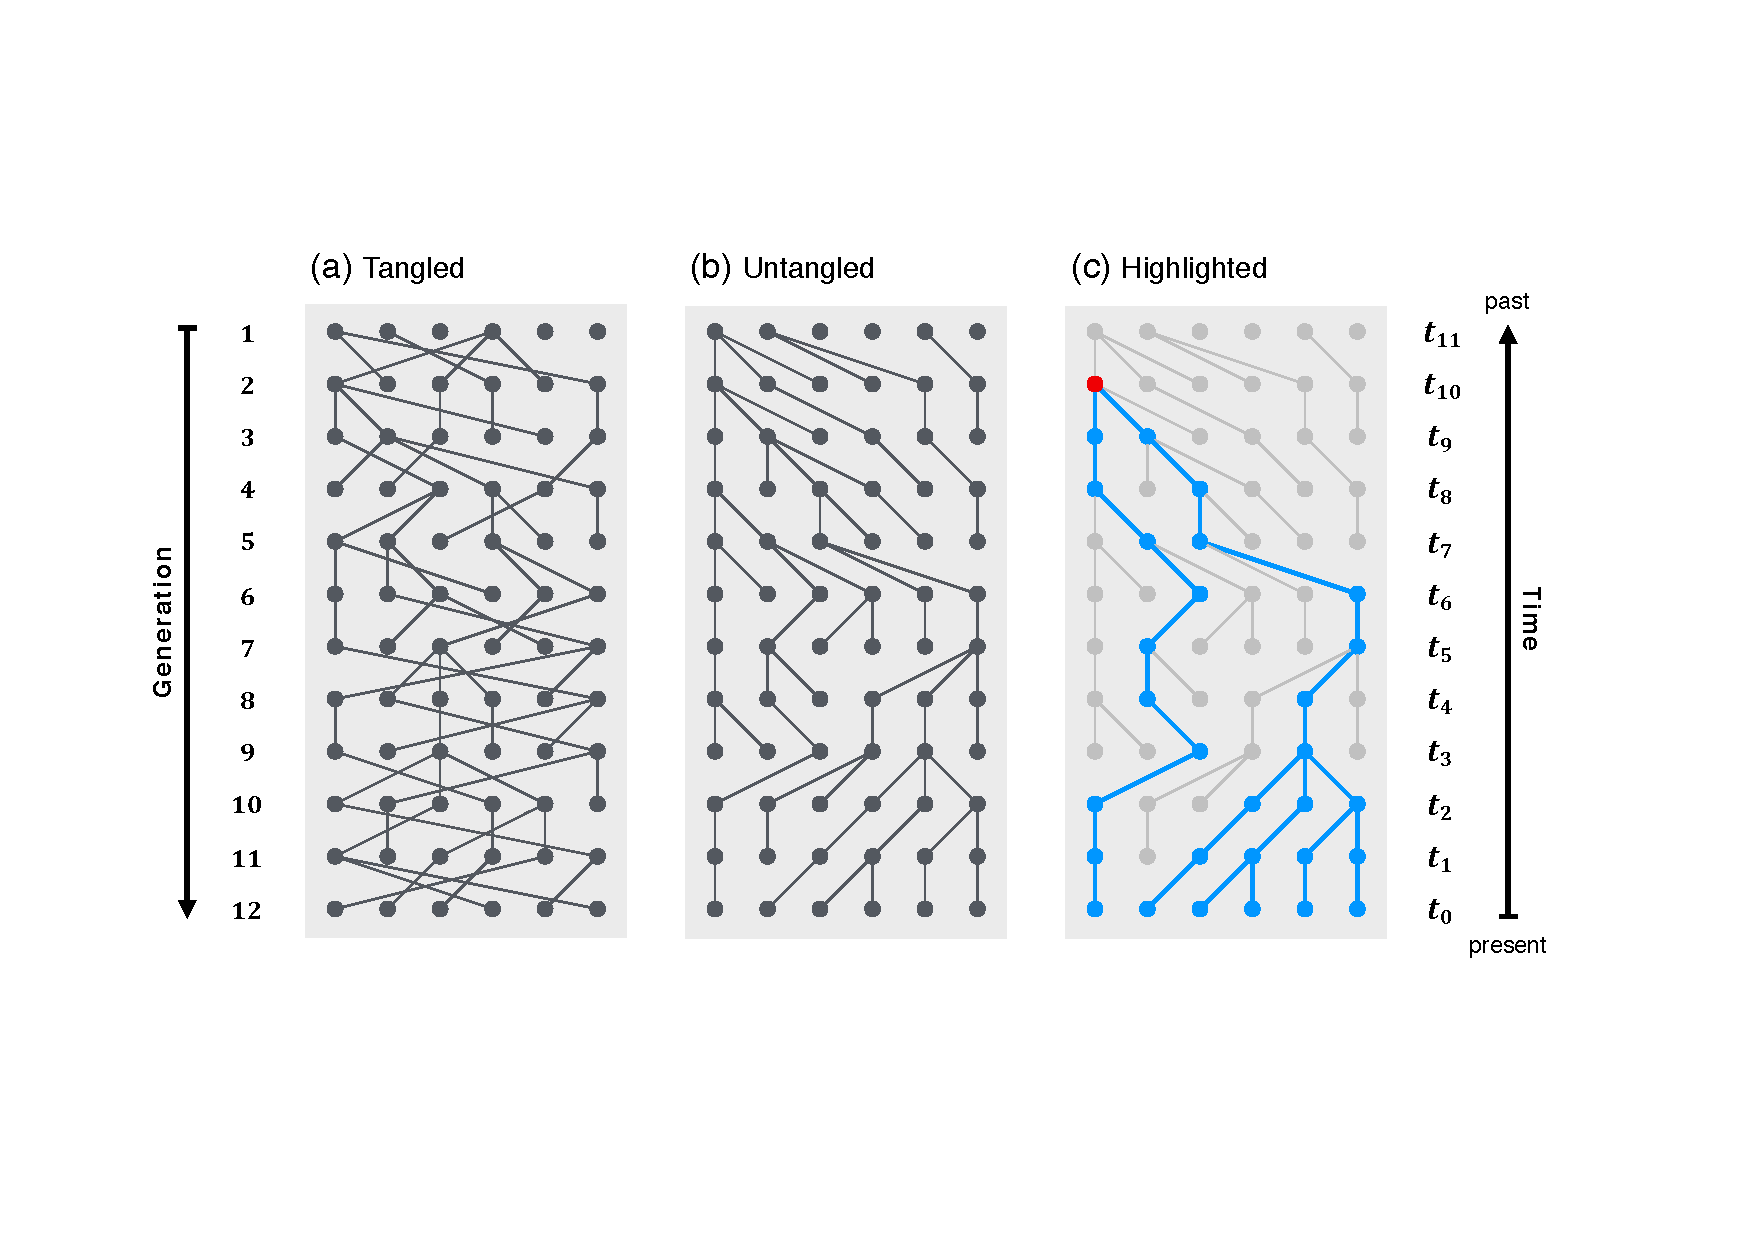
\includegraphics[width=\textwidth]{./img/ch1/info_wrightfisher}
\Caption{Example genealogy in a Wright-Fisher model}
{A population of size ${N=6}$ is shown in Panel~\textbf{(a)}, which is observed over 12 generations.
In the neutral Wright–Fisher model, \n{1} individual is chosen at random (with replacement) in each generation to produce offspring for the next generation, repeated $N$~times.
The genealogy of the population is more clearly seen after individuals have been sorted such that their lineages do not cross; see Panel~\textbf{(b)}.
Note that not every individual produces offspring, such that some lineages go extinct.
If this process is repeated over many generations (forward in time), it can be seen that all individuals in the present generation derive from a single individual in the past, which is indicated in Panel~\textbf{(c)}.
The ancestry of the present population (\emph{blue}) is traced back to a single ancestor (\emph{red}) at time ${t=10}$~generations ago.}
{fig:info_wrightfisher}
\end{figure}

%

In its simplest form, the Wright-Fisher model considers a gene locus at which \n{2} alleles, $A$~and~$a$, are observed; \ie the locus is \emph{biallelic}.
A population of $N$~haploid individuals is assumed, where $N$ remains constant in each generation.
All individuals die at the same time at which all individuals in the next generation are born; \ie time is measured in discrete, non-overlapping generations.
The effects of mutation or selection are ignored, such that alleles are \emph{neutral} and the probability to produce offspring is equal for each individual.
It follows that reproduction is considered as a random sampling process, in which the alleles that are transmitted into the next generation are drawn (with replacement) from the gene pool of the current population.
An example is illustrated in \cpref{fig:info_wrightfisher}.
% In respect to the genealogy of the population (\ref{fig:info_wrightfisher}{c}), implicitly, all individuals in the present generation will have descended from a single individual.
% Therefore, the genealogy of the Wright-Fisher model can be described
% as a coalescent process, which is further explained in \cpref{sec:coalescent}.

Since each draw has only \n{2} possible outcomes, $A$~or~$B$, each generation is produced by a series of independent Bernoulli trials such that allele frequencies are binomially distributed.
Let $X_t$ denote the number of $A$ alleles in generation $t$.
Given ${X_t=i}$ allele copies (or individuals which carry the allele),
the probability to draw the $A$ allele is equal to its frequency in the current generation, denoted by ${\pi_i = \rfrac{i}{N}}$.
The probability of observing ${X_{t+1}=j}$ copies in the next generation is
\begin{equation}\label{eq:WFprob}
	P(j \mid i) ~=~ {{N}\choose{j}} ~ \pi_i^j ~ (1 - \pi_i)^{N-j}
\end{equation}
for ${0 \leq i,j \leq N}$, and where ${\sum_{j=0}^{N} P(j \mid i) j = i}$.
From the binomial distribution follows that the expected value of the number of alleles in the next generation can be expressed as
\begin{equation}\label{eq:WFexp}
	\mathbb{E}[X_{t+1} \mid X_{t}] ~=~ N \pi_i ~=~ N \frac{X_t}{N} ~=~ X_t
\end{equation}
and the variance is given by
\begin{equation}\label{eq:WFvar}
	\operatorname{Var}[X_{t+1} \mid X_{t}] ~=~ N \pi_i (1 - \pi_i) ~=~ X_t \Big( 1 - \frac{X_t}{N} \Big)
	\ \text{.}
\end{equation}

\Cref{eq:WFexp} implies that ${\mathbb{E}[X_t] = \mathbb{E}[X_{t-1}]}$ and thereby ${\mathbb{E}[X_t] = \mathbb{E}[X_0]}$; \ie the expected number of alleles in each generation is (on average) equal to the initial allele count.
This result is reminiscent of the Hardy-Weinberg principle \citep{Hardy:1908wx,Weinberg:1908tr}, which states that the relative allele frequency remains constant in each generation if mating is random, but in which the population size is assumed to be infinite.
However, due to the behaviour of a stochastic process in a finite population, the number of allele copies may eventually \emph{drift} to $0$~or~$N$, even in a single generation.
Several examples of how the allele frequency may change in populations of different size are shown in \cpref{fig:wfsim}.

%
%!TEX root = ../../main.tex


\begin{figure}[!htb]
\centering
%\hrulefill \\
%\vspace{5pt}
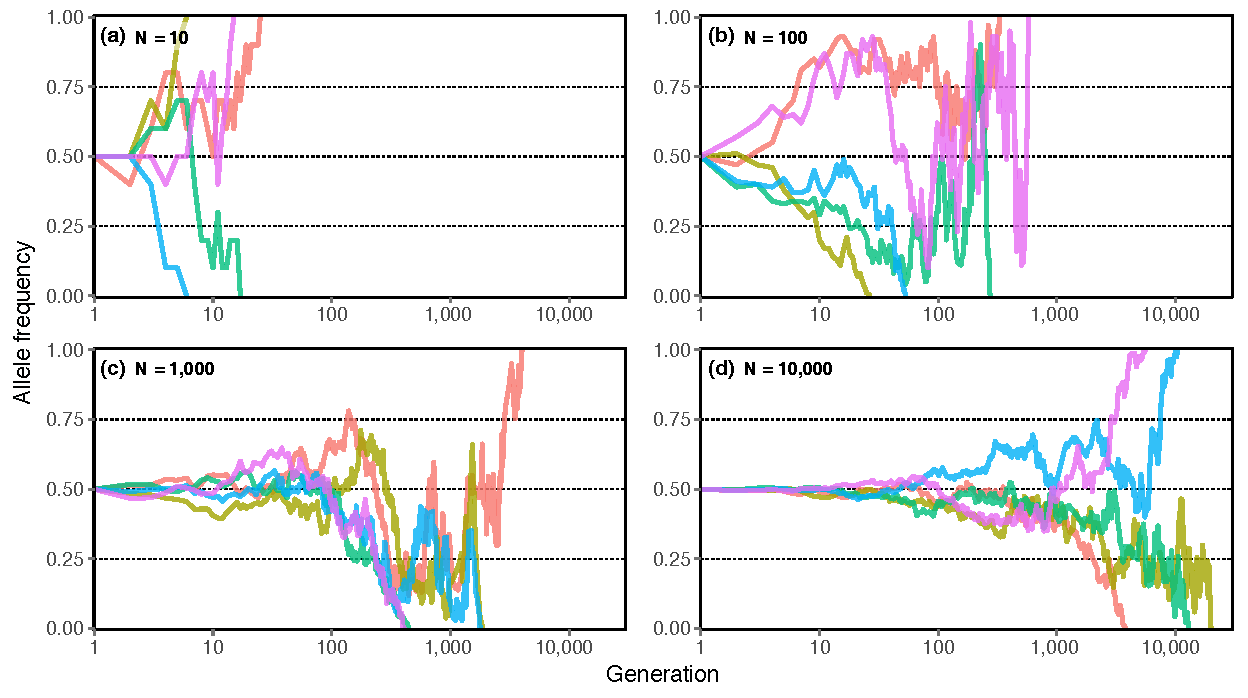
\includegraphics[width=\textwidth]{./img/ch1/wfsim}
\Caption{Allele frequency changes over time simulated under the Wright-Fisher model}
{A haploid population was simulated under \n{4} different constant values of population size, $N$, as indicated in each panel.
The change in allele frequency is shown by generation.
For each value of $N$, \n{5} replicate simulations were conducted (distinguished by colour).
Note that the allele frequency does not change after it has reached 0~or~1; \ie the allele is said to have become \emph{fixed} in the population.}
{fig:wfsim}
% \vspace{-5pt}
% \hrulefill%
\end{figure}

%

Because the frequency of an allele in a particular generation only depends on the frequency distribution in the previous generation, it follows from this property that the reproductive process is itself a Markov chain, with transition probabilities as described by \cref{eq:WFprob} and a state space in $\{0,\ldots,N\}$.
The states $0$ and $N$ are absorbing, which means that if the population consists of ${X_t=0}$ or ${X_t=N}$ alleles, it remains so in all future generations.
A consequence of this Markov process is that an allele will either go extinct or reach \emph{fixation} \citep[\eg, see][]{ewens2012}.
Let the time until either of the \n{2} alleles has reached fixation be denoted by $T$.
From \cref{eq:WFexp} follows that the probability that an allele reaches fixation is
\begin{equation}
	P(X_T \in \{0,N\}) = \frac{X_0}{N}
\end{equation}
which means that the probability of a given allele to reach fixation is equal to its initial frequency.

Without the introduction of new alleles through mutation, the Wright-Fisher model predicts that genetic variation is inevitably lost over time, due to random drift resulting from sampling error in a finite population. \label{ref:mutgendiv}
Hence, an important extension of the Wright-Fisher model is the incorporation of mutations.
Suppose that allele~$A$ mutates into allele~$a$ with rate~$\mu_A$, and $a$~into~$A$ with rate~$\mu_a$.
The transition probability given in \cref{eq:WFprob} still holds, but allele frequency can be expressed such that $\pi_i$ is dependent on the effect of mutation; see below.
\begin{equation}
	\pi_i ~=~ \frac{i}{N} ~ (1 - \mu_A) ~+~ \Big( 1 - \frac{i}{N} \Big) ~ \mu_a
\end{equation}
If ${\mu_A, \mu_a > 0}$, then transitions from any state into any other state remain possible in each generation and permanent fixation is avoided.
Note that in a population in which the effects of mutation and genetic drift are in statistical equilibrium allele frequencies are expected to follow the Hardy-Weinberg principle; \ie the population is in \gls{hwe}.

% TODO briefly outline Moran model
% \citep{Moran:1958cm}


%
\subsection{Coalescent theory}
\label{sec:coalescent}
%

The coalescent is arguably the most frequently employed genealogical method in population genetics.
The concept and the statistical properties of the coalescent were first described by \citet{Kingman:1982x,Kingman:1982gu,Kingman:1982uj} and it is therefore often referred to as ``Kingman's~coalescent''.
The term ``$n$-coalescent'' is also frequently used to emphasise the importance of the sample size, $n$, in the genealogical process within a much larger population.
The coalescent, at its core, is a collection of stochastic models which provide the means to generate predictions about population dynamics under a variety of models of genetic variation and demography \citet{wakeley2008}.
Note that the term ``prediction'' may sound odd given that the coalescent, by its very purpose, looks backward in time to reconstruct a possible genealogy given a set of population parameters.
The coalescent is often used to simulate the ancestry of a sample, from which particular model parameters can be inferred, for example, on basis of biological observations.
The first computational algorithm for simulations under the coalescent (named ``\emph{ms}'') was devised by \citet{Hudson:1990vob}.
Over the past decades, coalescent theory has grown extensively.
Hence, this section provides only a summary of the basic properties of the coalescent as relevant for this thesis.
For a more thorough presentation of the subject see, for example, \citet{Fu:1999fj}, \citet{neuhauser2001}, \citet{nordborg2001coalescent}, \citet{hein2004gene}, and \citet{wakeley2008}.


In contrast to the Wright-Fisher model, as well as other approaches which model the genealogical history of a population forward in time, the coalescent process reconstructs the genealogy of a sample by tracing the ancestry of individuals (or genes) backward in time.
Ancestral relationships between individuals are represented as lineages in a genealogical tree.
In each generation, each individual independently chooses \n{1} ancestor at random.
If \n{2} individuals choose the same ancestor by chance, their lineages are joined; \ie they \emph{coalesce}.
The time at which \n{2} lineages join is referred to as a \emph{coalescent~event}.
This process is repeated until only \n{1} lineage is left, which belongs to the \gls{mrca} of the sample.

%
%!TEX root = ../../main.tex


\begin{figure}[!htb]
\centering
%\hrulefill \\
%\vspace{5pt}
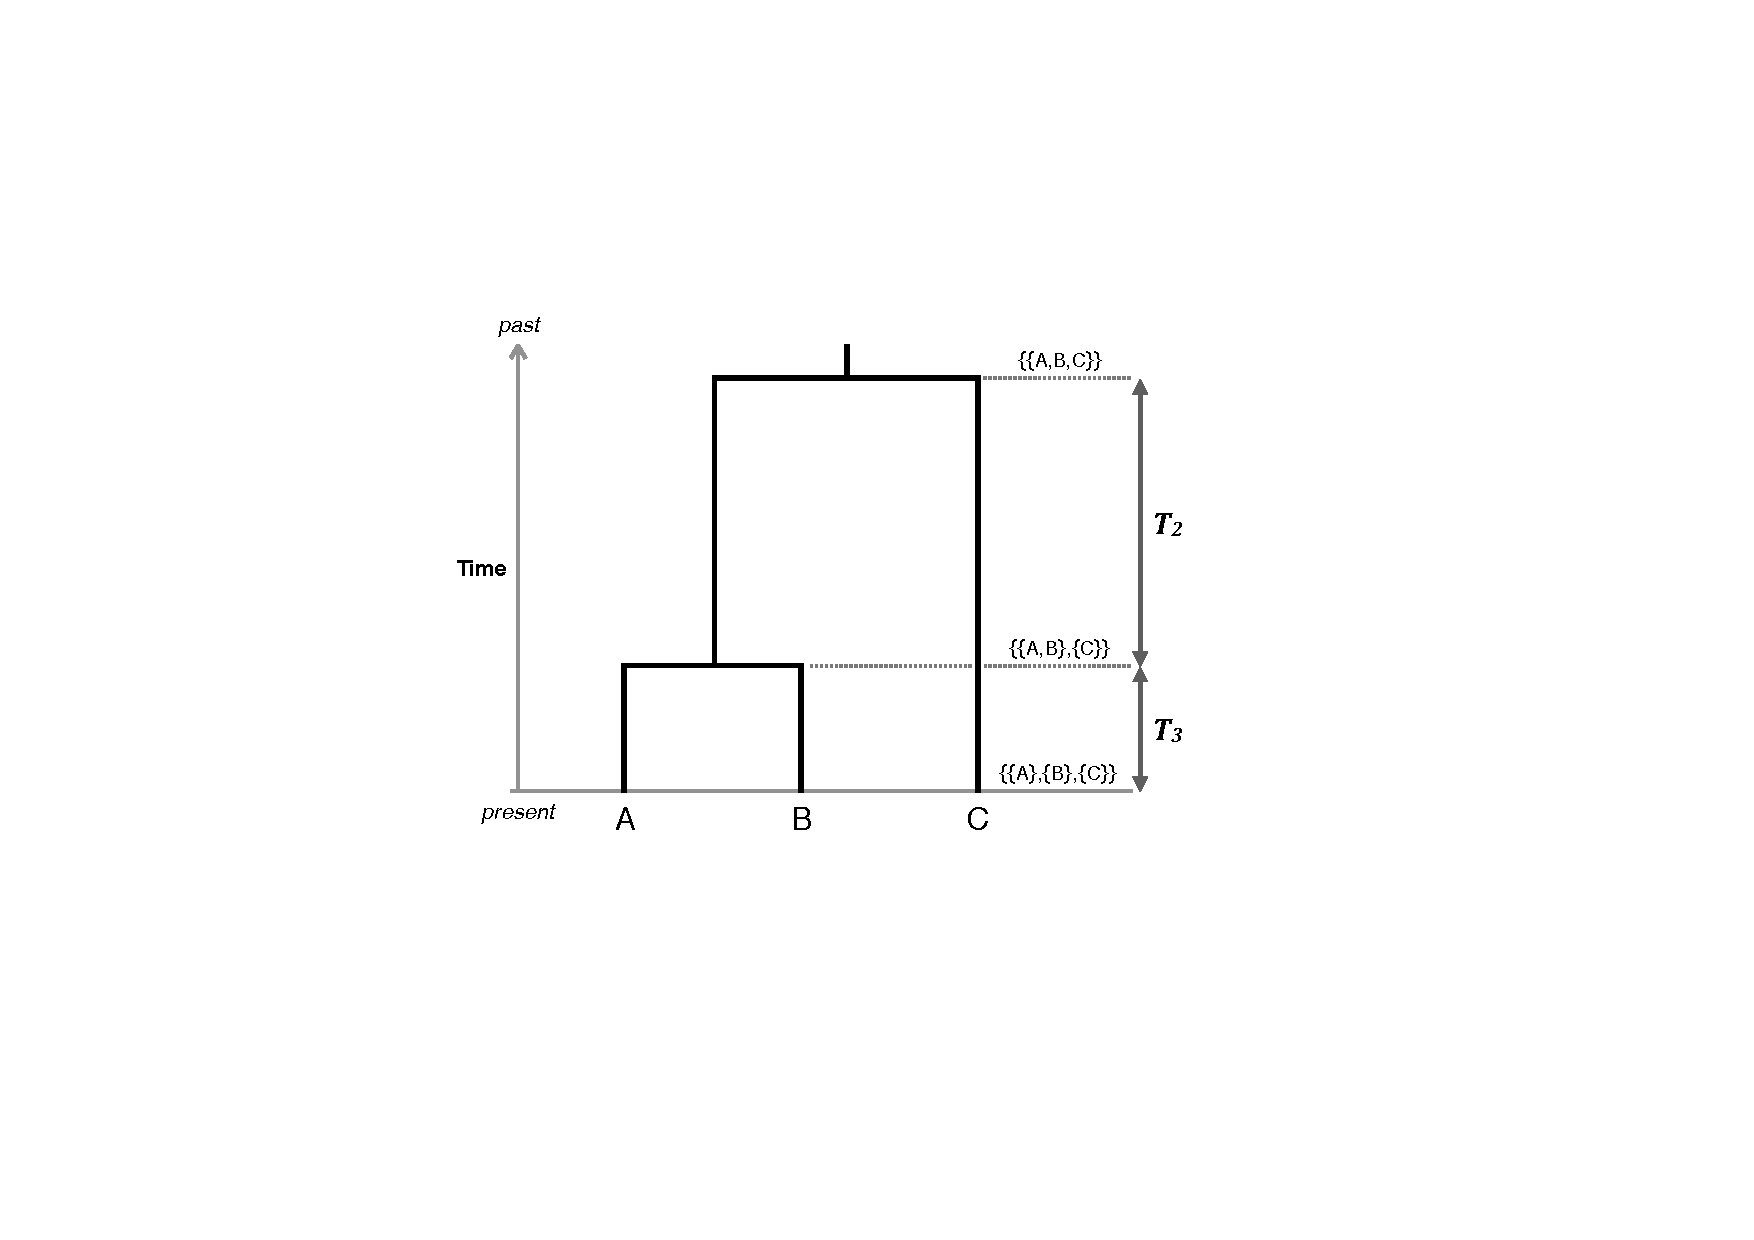
\includegraphics[width=0.7\textwidth]{./img/ch1/info_coalescent}
\Caption{Topology of a genealogical tree in the coalescent}
{The genealogical relationship of \n{3} haploid individuals is shown, $A$, $B$, and $C$, which represent separate lineages at present, but where $A$~and~$B$ are the first to coalesce (back in time).
The waiting time between successive coalescent events is denoted by \Correct{$T_j$}, where \Correct{$j$} is the number of ancestral lineages at a given time interval, which changes from \Correct{$j$} to \Correct{${j-1}$} at coalescence.
Figure modified from \citet{nordborg2001coalescent}.}
{fig:info_coalescent}
% \vspace{-5pt}
% \hrulefill%
\end{figure}

%

The history of a sample is reflected in its genealogy and can be described in terms of the topology of the tree and the lengths of the connecting branches.
The branch length corresponds to the time interval between \n{2} successive coalescent events, which is of central interest to describe the coalescent process.
Let this waiting time be denoted by $T_n$, where $n$ corresponds to the number of distinct lineages during the time interval, which changes from $n$ to ${n-1}$ at coalescence.
An example of a simple genealogical tree is shown in \cpref{fig:info_coalescent}, in which the waiting times between coalescent events are indicated.
In the following, the concept of the standard coalescent is described by assuming a haploid population of constant size, $N$, in which the effects of mutation, selection, recombination, or other biological processes are not involved.

For now, consider a sample of ${n=2}$ individuals taken at the present time, which are followed back in time until the first coalescent event.
Since there are $N$ possible ancestors, the probability that a particular ancestor is chosen by \n{1} of the individuals is equal to $N^{-1}$.
The probability that \n{2} individuals choose the same ancestor independently is $N^{-2}$.
Hence, the probability that any of the possible ancestors is chosen by \n{2} individuals is equal to ${N \times N^{-2} = N^{-1}}$, and the probability that none is chosen is ${1 - N^{-1}}$.
To arrive at the probability that \n{2} lineages coalesce $t>0$ generations back in time, it is implied that they do not choose the same ancestor in previous generations.
Because generations are independent, the probability that the \n{2} lineages are distinct over $t-1$~generations is
\begin{equation}
	P(T_2 > t \mid N) ~=~ \Big( 1 - \frac{1}{N} \Big)^{t-1}
	\ \text{.}
\end{equation}
Therefore, the probability that \n{2} lineages coalesce $t$ generations back in time is geometrically distributed with rate $N^{-1}$, such that
\begin{equation}\label{eq:coalprob}
	P(T_2 \geq t \mid N) ~=~ \Big( 1 - \frac{1}{N} \Big)^{t-1} ~ \frac{1}{N}
\end{equation}
which arises from the number of independent Bernoulli trials needed until the same ancestor is chosen by \n{2} lineages.
It follows from the geometric distribution that the expected number of generations up to and including the coalescent event is
\begin{equation}\label{eq:coal_2_exp}
	\mathbb{E}[T_2 \mid N] ~=~ \frac{1}{N^{-1}} ~=~ N
\end{equation}
and the variance is
\begin{equation}\label{eq:coal_2_var}
	\operatorname{Var}[T_2 \mid N] ~=~ \frac{1 - N^{-1}}{N^{-2}} ~=~ N^2 ~ \Big( 1 - \frac{1}{N} \Big)
	\ \text{.}
\end{equation}

A notable result is that the expected time to the first coalescent event is equal to the size of the population; see \cref{eq:coal_2_exp}.
It is therefore convenient to scale time in units of $N$~generations, namely
\begin{equation}\label{eq:timescale}
	\tau ~=~ \frac{t}{N}
\end{equation}
where the time, $\tau$, is continuous (as opposed to time measured in distinct generations) and referred to as the \emph{population-scaled} time.
The probability that a pair of lineages remains distinct during a given time interval is given below, but which can now be approximated using the exponential distribution if the population size is sufficiently large, \ie as $N$ tends to infinity;
\begin{equation}\label{eq:coal_2_dont}
	P(T_2 > \tau \mid N)
	~=~ \Bigg( 1 - \frac{1}{N} \Bigg)^{\lfloor N \tau \rfloor}
	\quad \xrightarrow{~ N~\rightarrow~\infty ~} \quad
	\euler{-\tau}
\end{equation}
where ${\lfloor N \tau \rfloor}$ is the largest integer that does not exceed ${N \tau}$ \citep[\eg, see][]{nordborg2001coalescent}.
% Likewise, the probability that the \n{2}~lineages coalesce is
% \begin{equation}\label{eq:coal_2_do}
% 	P(T_2 \geq \tau \mid N)
% 	~=~ \Bigg( 1 - \frac{1}{N} \Bigg)^{\lfloor N \tau \rfloor} \frac{1}{N}
% 	\quad \xrightarrow{~ N~\rightarrow~\infty ~} \quad
% 	\frac{1}{N} \euler{-\tau}
% 	\ \text{.}
% \end{equation}
% Since the scaled time to coalescence for \n{2} individuals is exponentially distributed, it follows that ${\mathbb{E}[T_2] \approx 1}$ and ${\operatorname{Var}[T_2] \approx 1}$.

The above can now be extended to consider $n$~lineages, which in the previous generation may have $n$ distinct ancestral lineages if no coalescent event has occurred, or ${n-1}$ otherwise.
The probability of no coalescence at a given time can be derived as follows.
Let the first lineage choose among $N$~ancestors with probability ${\rfrac{N}{N} = 1}$, the second lineage then chooses among the remaining ${N-1}$ ancestors with probability ${\rfrac{N-1}{N}}$, the third chooses among ${N-2}$ ancestors with probability ${\rfrac{N-2}{N}}$, and so on; \ie
\begin{equation*}
	\Big(\frac{N}{N}\Big) ~ \Big(\frac{N-1}{N}\Big) ~ \Big(\frac{N-2}{N}\Big) ~ \cdots ~ \Big(\frac{N-(n-1)}{N}\Big)
\end{equation*}
which is equal to
\begin{equation}\label{eq:coal_n_dont}
	\prod_{k=0}^{n-1} \frac{N-k}{N}
	~=~ \prod_{k=1}^{n-1} \Big( 1 - \frac{k}{N} \Big)
	~=~ 1 - {n \choose 2} \frac{1}{N} ~+~ \mathcal{O}\Big( \frac{1}{N^{2}} \Big)
\end{equation}
where the binomial coefficient, ${{n \choose 2} = \sum_{k=1}^{n-1}k}$, corresponds to the number of possible pairs.
Similarly, the probability that any \n{2} of the $n$~lineages coalesce at a given time implies that the remaining lineages do not coalesce, therefore
\begin{equation}\label{eq:coal_n_do}
\begin{split}
	P(T_n = \tau \mid N)
	& ~=~ {n \choose 2} \frac{1}{N} ~\times~ \Big(1-\frac{1}{N}\Big) ~ \Big(1-\frac{2}{N}\Big) ~ \cdots ~ \Big(1-\frac{n-2}{N}\Big) \\
	& ~=~ {n \choose 2} \frac{1}{N} ~\times~ \prod_{k=1}^{n-2} \Big( 1 - \frac{k}{N} \Big) \\
	& ~=~ {n \choose 2} \frac{1}{N} ~+~ \mathcal{O}\Big( \frac{1}{N^{2}} \Big)
	\ \text{.}
\end{split}
\end{equation}
Note that the term ${\mathcal{O}(N^{-2})}$ describes the limiting behaviour of \cref{eq:coal_n_dont,eq:coal_n_do} and captures all terms that decrease more rapidly than $\rfrac{1}{N}$ as $N$ tends to infinity.
Mathematically, ${\mathcal{O}(N^{-2})}$ corresponds to the \emph{diffusion} limit of the continuous process, which can be ignored if the population size is sufficiently large \citep[\eg, see][]{wakeley2008}.
By doing so, it is assumed that not more than \n{2} lineages coalesce at a given time, such that the resulting tree has a binary topology.
% This assumption differs from the Wright-Fisher model, where any individual may have multiple offspring such that $n$~lineages may have ${1,2,\ldots,n}$ ancestors in the immediately previous generation.
In the limit, and if ${n \ll N}$, the probability of a coalescent event at a given time is
\begin{equation}\label{eq:coal_approx}
	P(T_n = \tau \mid N) ~\approx~ {n \choose 2} \frac{1}{N}
\end{equation}
and, as before, the waiting time can be approximated in terms of the exponential distribution as given below.
\begin{equation}\label{eq:coal_n_approx}
	P(T_n > \tau \mid N)
	~\approx~ \Bigg( 1 - {n \choose 2} \frac{1}{N} \Bigg)^{\lfloor N \tau \rfloor}
	\quad \xrightarrow{~ N~\rightarrow~\infty ~} \quad
	\euler{-{n \choose 2}\tau}
\end{equation}
Thus, in the continuous-time coalescent, the approximate waiting time between successive coalescent events, $T_n$, is exponentially distributed with rate ${n \choose 2}$, from which follows that the expected value is
\begin{equation}\label{eq:coal_n_exp}
	\mathbb{E}[T_n] ~=~ \frac{1}{{n \choose 2}} ~=~ \frac{2}{n(n-1)}
\end{equation}
and the variance is
\begin{equation}\label{eq:coal_n_var}
	\operatorname{Var}[T_n] ~=~ \frac{1}{{n \choose 2}^2} ~=~ \frac{4}{n^2 (n-1)^2}
	\ \text{.}
\end{equation}
% It has been shown that the approximate probability of coalescence from \cref{eq:coal_n_approx} is highly accurate, even under biologically realistic values of $N$.
% For example, in comparison to the exact probability from \cref{eq:coal_n_do}, the calculated difference is less than 0.5\% at a sample size of ${N=\num{10000}}$ \citep{wakeley2008}.
%the coalescent converges to the ancestral process of the Wright-Fisher model


An important result of the coalescent is that an expectation for the \gls{tmrca} can be derived dependent on the population size.
Given the sum of branch lengths that need to be traced back to arrive at the \gls{mrca},
\begin{equation*}
	T_\text{MRCA} ~=~ T_N + T_{N-1} + \dots + T_2
\end{equation*}
the expected value can be expressed as
\begin{equation}\label{eq:coal_tmrca}
	\mathbb{E}[T_\text{MRCA} \mid N]
	~=~ \sum_{n = 2}^{N} \mathbb{E}[T_n]
	~=~ \sum_{n = 2}^{N} \frac{2}{n(n-1)}
	~=~ 2~\Big( 1 - \frac{1}{N} \Big)
	\ \text{.}
\end{equation}
Therefore, ${\mathbb{E}[T_\text{MRCA}] \approx 2}$ as ${N\rightarrow\infty}$, which implies that on average the number of generations until the entire sample has coalesced into a single ancestral lineage is equal to about twice the population size.


%
\subsubsection{Effective population size}
%

Natural populations rarely adhere to the assumptions made by mathematical models.
One such example is the rather unrealistic assumption that the population size remains constant over time.
The rate at which coalescent events occur in the genealogy of a sample is conditional on the size of the population in each generation, which in reality is often highly variable.
Statistical models in population genetics may therefore resort to the concept of an effective population size, denoted by \Ne, which substitutes the census population size, $N$, to account for departures from model assumptions.
Note that the biological meaning and the mathematical definition of \Ne may vary depending on the properties of the biological system under consideration.
To account for variations in population size in the standard coalescent, \Ne can be defined as the \emph{variance effective size} and is estimated such that the coalescent process would result in the same shape of genetic variation as expected in a population of constant size.

Note that \Ne may differ from the census size of a population by several magnitudes.
For example, the human population currently counts several billion individuals globally, whereas the long-term, diploid effective size is commonly defined in the order of ${\Ne \approx \num{10000}}$, based on estimates from \gls{dna} polymorphism data \citep[\eg][]{Takahata:1993ko,Yu:2001wl}.

Suppose the size of a population is known at each generation back time, where $N_i$ denotes the census size in generation~$i$ over a period of $t$ discrete generations.
The effective size can be computed as
\begin{equation}
	\Ne ~=~ \frac{t}{ \sum_{i=1}^{t} \frac{1}{N_i} }
\end{equation}
which is the harmonic mean of $N_i$.
However, because past population sizes are typically difficult to assess, \Ne can be estimated from the genetic diversity observed in a population.
The measure of genetic diversity is dependent on the rate of mutation in the genome, which is described in the following section\label{ref:calceffpopsize}.
For consistency with the definitions provided so far, the following sections in this chapter keep $N$ to denote the population size, but which is substituted by \Ne in the remaining chapters.


%
\subsubsection{The coalescent with mutation}
\label{sec:coal_mutation}
%

Mutations are essential to generate genetic diversity and maintain genetic variation in a finite population.
The standard coalescent relies on the assumption that variant alleles are selectively neutral; \ie the effect of mutation is independent of the genealogical process.
As such, mutation events can be superimposed on the coalescent tree by placing mutations on all branches proportional to their length.
An example is illustrated in \cpref{fig:info_mutation}, in which several mutation events are shown to give rise to the variation observed in the \gls{dna} sequence of a sample.

%
%!TEX root = ../../main.tex


\begin{figure}[!htb]
\centering
%\hrulefill \\
%\vspace{5pt}
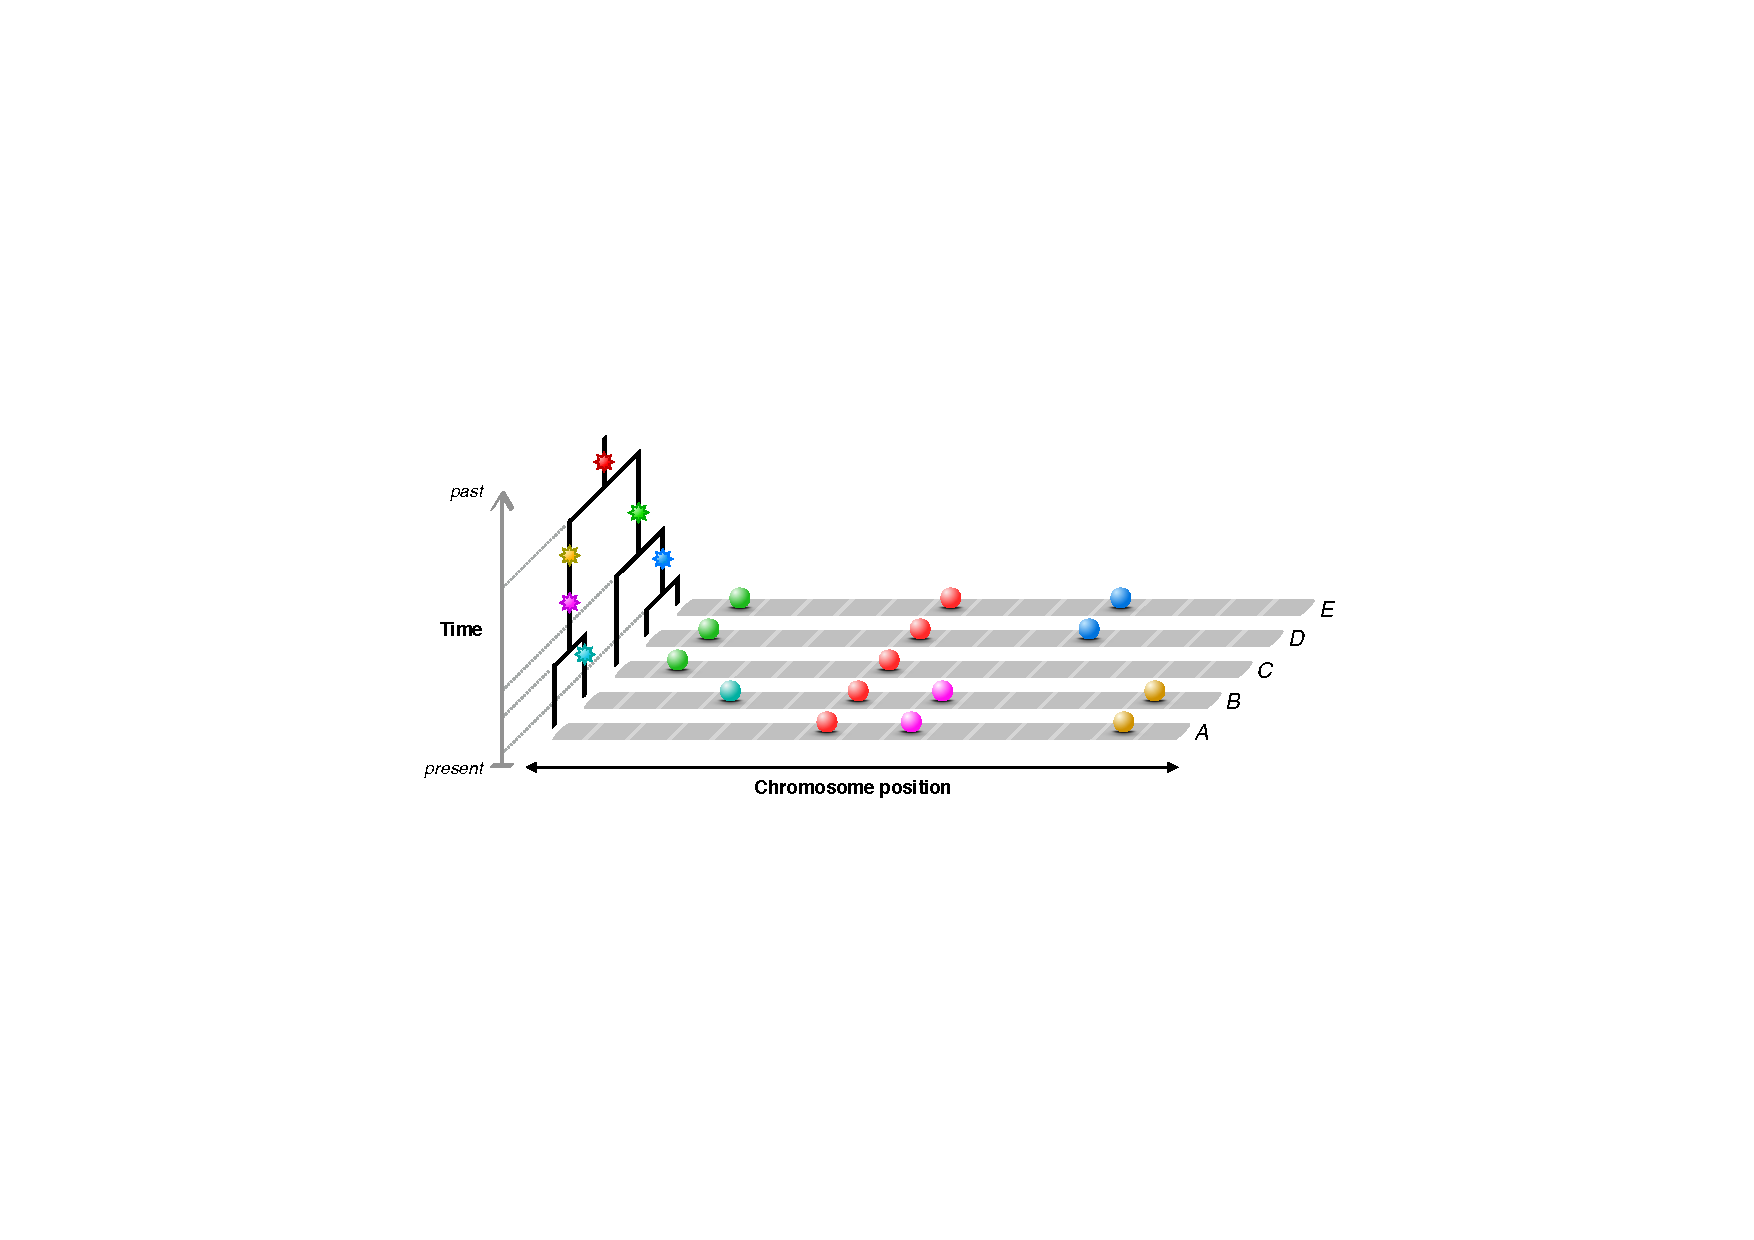
\includegraphics[width=\textwidth]{./img/ch1/info_mutation}
\Caption{Mutation events on a genealogical tree in the coalescent}
{The genealogy of a sample of \n{5} haploid individuals ($A-E$) is shown on the left.
The time of each coalescent event is indicated by a \emph{dotted} line.
Mutation events (\emph{stars}) are placed along the branches of the tree.
Each mutation event alters the allelic state at a random position on the chromosome, giving rise to a new allele, which is inherited by all descendants of the ancestral individual in which the mutation occurred.
Horizontal lanes (\emph{grey}) represent the chromosome sequence of the individuals, on which the derived alleles are depicted as \emph{marbles}; colours correspond to the mutation event from which the alleles derive.}
{fig:info_mutation}
% \vspace{-5pt}
% \hrulefill%
\end{figure}

%

Given a constant rate of mutation per site per generation, $\mu$, the expected number of mutations on a branch in the genealogical tree, \ie a lineage that is $t$~generations long, is ${t\mu}$.
If time is scaled in units of $N$~generations, see \ctref{eq:timescale}, the corresponding value is expressed by ${\tau N \mu}$, such that the rate of mutation per site per unit of time is equal to ${N \mu}$.
However, for historical reasons \citep[\eg, see][]{wakeley2008}, the population-scaled mutation rate is given by the compound parameter
\begin{equation}\label{eq:mutrate}
	\theta = 2 N \mu
\end{equation}
where $\theta$ is assumed to be constant in the limit ${N\rightarrow\infty}$.
Note that the factor of 2 relates to the formulation of the expected number of pairwise differences between \n{2} haploid sequences, which is equal to $\theta$ \citep{tajima1993}.
Thus, $\theta$ describes the amount of genetic diversity in a population.

Because mutations effectively count events that occur independently, the probability distribution of mutation is described by a Poisson process with rate parameter ${\rfrac{\theta}{2}}$ \citep{wakeley2008}.
It follows that the probability to observe $K$ mutations on a branch of length~$L$ is itself Poisson distributed with parameter ${\rfrac{\theta L}{2}}$;
\begin{equation}
	P(K = k \mid L) ~=~ \bigg( \frac{\theta L}{2} \bigg)^k ~ \frac{1}{k!} \euler{-\frac{\theta L}{2}}
\end{equation}
where ${L=t}$ if measured in discrete generations or ${L=N\tau}$ if measured on a continuous time scale.
It follows from the Poisson distribution that ${\mathbb{E}[K \mid L] ~=~ \operatorname{Var}[K \mid L] ~=~ \rfrac{\theta L}{2}}$.

Suppose that each mutation event creates a new allele and that each site can only mutate once in the history of the sample; such a setting is generally referred to as the infinite sites model \citep{Kimura:1969tn,Watterson:1975ura}.
Under this assumption, the number of segregating sites (or \emph{variant} sites) observed in sequence data in a sample of size~$n$, is equal to the sum of mutation events that occurred in the history of the sample.
The total branch length of the tree thereby determines the expected value of the number of segregating sites, denoted by $S_n$.
From the sum of all branch lengths, \ie
\begin{equation*}
	T_\text{total} ~=~ i T_i ~+~ (i-1) T_{i-1} ~+~ (i-2) T_{i-2} ~+~ \ldots ~+~ 2 T_2
\end{equation*}
where $i$ is the number of distinct lineages during a given time interval,
the expected value of the total branch length can be computed as
\begin{equation}
	\mathbb{E}[T_\text{total}]
	~=~ \sum_{i=2}^{n} i ~ \mathbb{E}[T_i]
	~=~ \sum_{i=2}^{n} i ~ \frac{2}{i(i-1)}
\end{equation}
where ${\mathbb{E}[T_i]}$ is given by \ctref{eq:coal_n_exp}.
From the above, the expected value of $S_n$ can be derived as follows.
\begin{equation}
	\mathbb{E}[S_n]
	~=~ \frac{\theta}{2} ~ \mathbb{E}[T_\text{total}]
	~=~ \frac{\theta}{2} \sum_{i=2}^{n} i ~ \frac{2}{i(i-1)}
	~=~ \theta \sum_{i=1}^{n-1} \frac{1}{i}
\end{equation}
%see \citet{Watterson:1961hv}.
By rearrangement, the following equation can be obtained;
\begin{equation}\label{eq:theta_w}
	\hat{\theta}_W = \frac{S_n}{\sum_{i=1}^{n-1} \frac{1}{i}}
\end{equation}
which is an unbiased estimator of the genetic diversity in sample of sequence data; also known as Watterson's $\theta$ \citep{Watterson:1975ura}.
With regard to the calculation of the effective population size as described in the previous section (\pref{ref:calceffpopsize}), it can be seen that an estimate for the value of \Ne can be obtained, for example, from \cref{eq:mutrate,eq:theta_w} given an estimate of the mutation rate.


%
\subsubsection{The coalescent with recombination}
%

Recombination is ubiquitous in nature and crucially involved in the spread of genetic variability in populations of sexually reproducing organisms.
\Citet{Hudson:1983vs} showed that the genealogical process in the coalescent can be extended to model recombination along the sequence of a sample.
In contrast to mutation events, which do not affect the topology of a tree under the standard coalescent, recombination events have a considerable effect on the structure of the genealogy.

Consider the sequence of \n{1} of the chromosomes present in a diploid individual.
Due to recombination, the different parts along the chromosome can be traced back to the ancestral material in \n{2} parents in the immediately previous generation, and further to \n{4} grandparents in the second previous generation, and so on.
It becomes clear that the ancestral origin of the chromosomal sequence is distributed over many parallel lineages back in time.
For example, a useful (but limited) representation of this process is seen in family trees (\emph{pedigrees}) in which ancestral lineages \emph{branch} back in time such that the number of ancestors appears to double in each generation.
Obviously, this progression cannot go on indefinitely because in a finite population any individual will be to some degree related to any other individual (their pedigrees may partially share the same ancestors).
As shown by \citet{Wiuf:1997wf}, all chromosomal lineages will eventually coalesce back onto a single lineage which is the \emph{ultimate} \gls{mrca} of the chromosomal sequence.

The coalescent with recombination includes coalescent events as well as branching events, but where the genealogy of a sample of sequences cannot be represented by a single tree.
This is because recombination alters the genealogical relation between different segments of the ancestral material such that \n{2} chromosomes may be closely related at a particular segment, but distantly related at another segment.
The chromosomal sequence is superimposed by a sequence of \emph{marginal} trees of different topology.
This tree sequence can be represented in a graph structure.
The most common way to represent the genealogy of a sample of sequences is the \gls{arg} which was first described by \citet{Griffiths:1991jp} in a \n{2}-locus model, but which was later generalised by \citet{Griffiths:1996dx,griffiths1997} in regards to the infinite sites model.
\Cpref{fig:info_arg} illustrates a minimal example of an \gls{arg} for a sample of \n{4}~chromosomes, in which mutation events are included to emphasise the pattern of allelic variation resulting from recombination between \n{2} loci.
In the following, the basic properties of the generalised \gls{arg} are presented.

%
%!TEX root = ../../main.tex


\begin{figure}[!htb]
\centering
%\hrulefill \\
%\vspace{5pt}
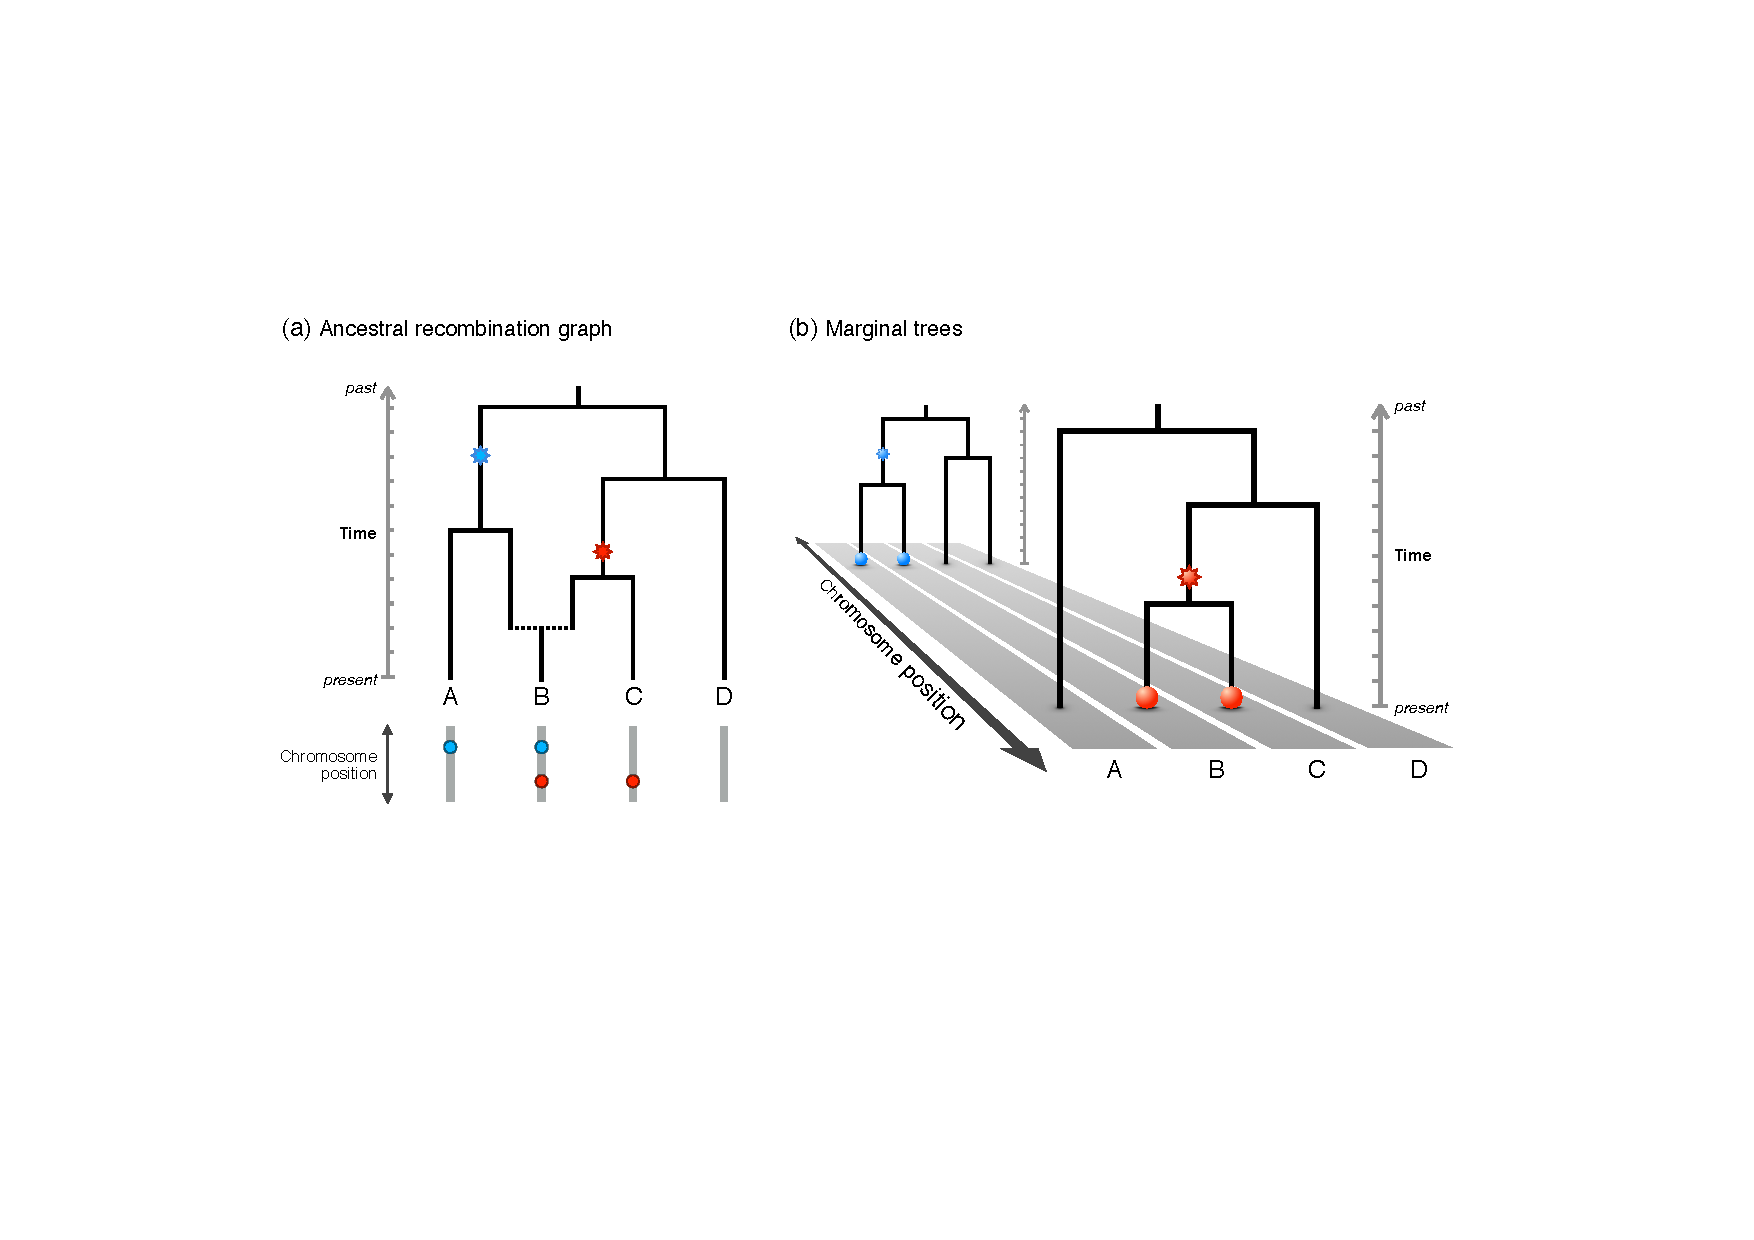
\includegraphics[width=\textwidth]{./img/ch1/info_arg}
\Caption{Illustration of the ancestral recombination graph}
{Panel~\textbf{(a)} shows the \gls{arg} for a sample of \n{4}~chromosomes, labelled by $A$, $B$, $C$, and $D$.
The \emph{dotted} horizontal line denotes the time of a recombination event between chromosomal lineages.
Mutation events are shown as \emph{stars}.
The chromosomal positions of derived alleles are indicated below the \gls{arg}.
The corresponding marginal trees are shown in Panel~\textbf{(b)}, where each lane (\emph{grey}) represents the chromosomal sequence on which the derived alleles sit (shown as \emph{marbles}).}
{fig:info_arg}
% \vspace{-5pt}
% \hrulefill%
\end{figure}

%

Given the rate of recombination per site per generation, $\rho$, the population-scaled recombination rate is given by the compound parameter
\begin{equation}\label{eq:recrate}
	\phi = 4 N \rho
\end{equation}
which is assumed to be constant in the limit ${N\rightarrow\infty}$.
The factor of 4 results from time being scaled in units of ${2 N}$ generations, accounting for the fact that the population is diploid.
Note that this adjustment permeates the coalescent and implies similar changes in other equations.
For example, the scaled mutation rate given in \ctref{eq:mutrate} needs to be written as $~{\theta = 4 N \mu}~$ if considered in a diploid population.

Given a sample of $n$~chromosomes, the number of chromosomal lineages, $k$, may increase (due to recombination) or decrease (due to coalescence) back in time.
First, consider the event of no recombination and no coalescence; \ie the value of $k$ remains the same in the previous generation \citep[\eg, see][]{tavare2004}.
The probability of this event is
\begin{equation}\label{eq:coalrec_dont1}
	(1 - \rho)^k ~\times~ \Big( 1 - \frac{1}{N} \Big) ~\times~ \Big( 1 - \frac{2}{N} \Big) ~\times~ \cdots ~\times~ \Big( 1 - \frac{k -1}{N} \Big)
\end{equation}
where ${(1 - \rho)^k}$ corresponds to the probability that none of the lineages recombine; the other terms refer to the probability of no coalescence, which was already defined in \ctref{eq:coal_n_dont}.
Now, because the rate at which \n{1} lineage branches into \n{2} lineages back in time is equal to $\rfrac{\phi}{2}$, \Cref{eq:coalrec_dont1} can be written as
\begin{equation}\label{eq:coalrec_dont2}
	1 - \frac{k\phi}{2N} ~-~ 1 - {k \choose 2}\frac{1}{N} ~+~ \mathcal{O}\Big( \frac{1}{N^2} \Big)
	\ \text{.}
\end{equation}
For the event ${k \rightarrow k+1}$, which can only be facilitated through recombination, it follows that the probability of a recombination event in the previous generation is given by
\begin{equation}
	\frac{k\phi}{2N} ~+~ \mathcal{O}\Big( \frac{1}{N^2} \Big)
	\ \text{.}
\end{equation}
The term ${\mathcal{O}(N^{-2})}$ is the diffusion limit of the function and corresponds to the probability that more than \n{1} recombination event occurs at a given unit of time, which can be ignored for larger population sizes; \ie as $N$ tends to infinity.
Similarly, a coalescent event in the previous generation means that ${k \rightarrow k-1}$, for which the probability has already been described in \ctref{eq:coal_approx}.
Also, as shown in \ctref{eq:coal_n_approx}, the probability of coalescent events, in the limit ${N\rightarrow\infty}$, is exponentially distributed with rate
\begin{equation}
	{k \choose 2} ~=~ \frac{k(k-1)}{2}
	\ \text{.}
\end{equation}
Likewise, in the limit, recombination follows the same distribution in the coalescent at rate
\begin{equation}
	\frac{k\phi}{2}
	\ \text{.}
\end{equation}

It follows that the coalescent with recombination can be described as a continuous-time Markov chain with a \emph{birth-death} process.
Lineages are ``born'' through recombination or ``die'' due to coalescence backward in time \citep[\eg, see][]{tavare2004,wakeley2008}.
The state space is delimited by ${k=n}$ at present and ${k=1}$ at an \gls{mrca}.
The transition rates can be summarised as follows.
\begin{equation}
k ~\rightarrow~
\renewcommand{\arraystretch}{1.2}
\left\{
\begin{array}{llll}
	k - 1  &  \text{at rate} & \rfrac{k(k-1)}{2} & \text{if lineages coalesce} \\
  k + 1  &  \text{at rate} & \rfrac{k\phi}{2}  & \text{if lineages recombine}
\end{array}
\right.
\end{equation}
Importantly, because the rate of coalescence is quadratic in the number of lineages and the rate of recombination is at most linear, the number of lineages cannot increase indefinitely \citep{Wiuf:1997wf}.
As a result, the ancestry of all chromosomal segments are eventually traced back to a single ancestral chromosome in the ultimate \gls{mrca}.

% TODO extend the coalescent with recombination by  a few more properties
% TODO mention other processes in the coalescent; eg selection (ASG) and migration


%
\subsection{Identity by descent}
%

% The concept of genetic inheritance
%
% \N{2} alleles are identical by descent if they were inherited from a common ancestor.
% Note that \n{2} alleles may be different due to mutation, despite being inherited from a common ancestor.

% When the DNA sequences of \n{2} individuals are compared, they may share an identical set of alleles \gls{ibs}
% \N{2} individuals may share a segment of identical DNA
% IBD is distinguished from \gls{ibs}

%
% %!TEX root = ../../main.tex


\begin{figure}[p]
{\small\texthv{\textbf{(a)}}} \\
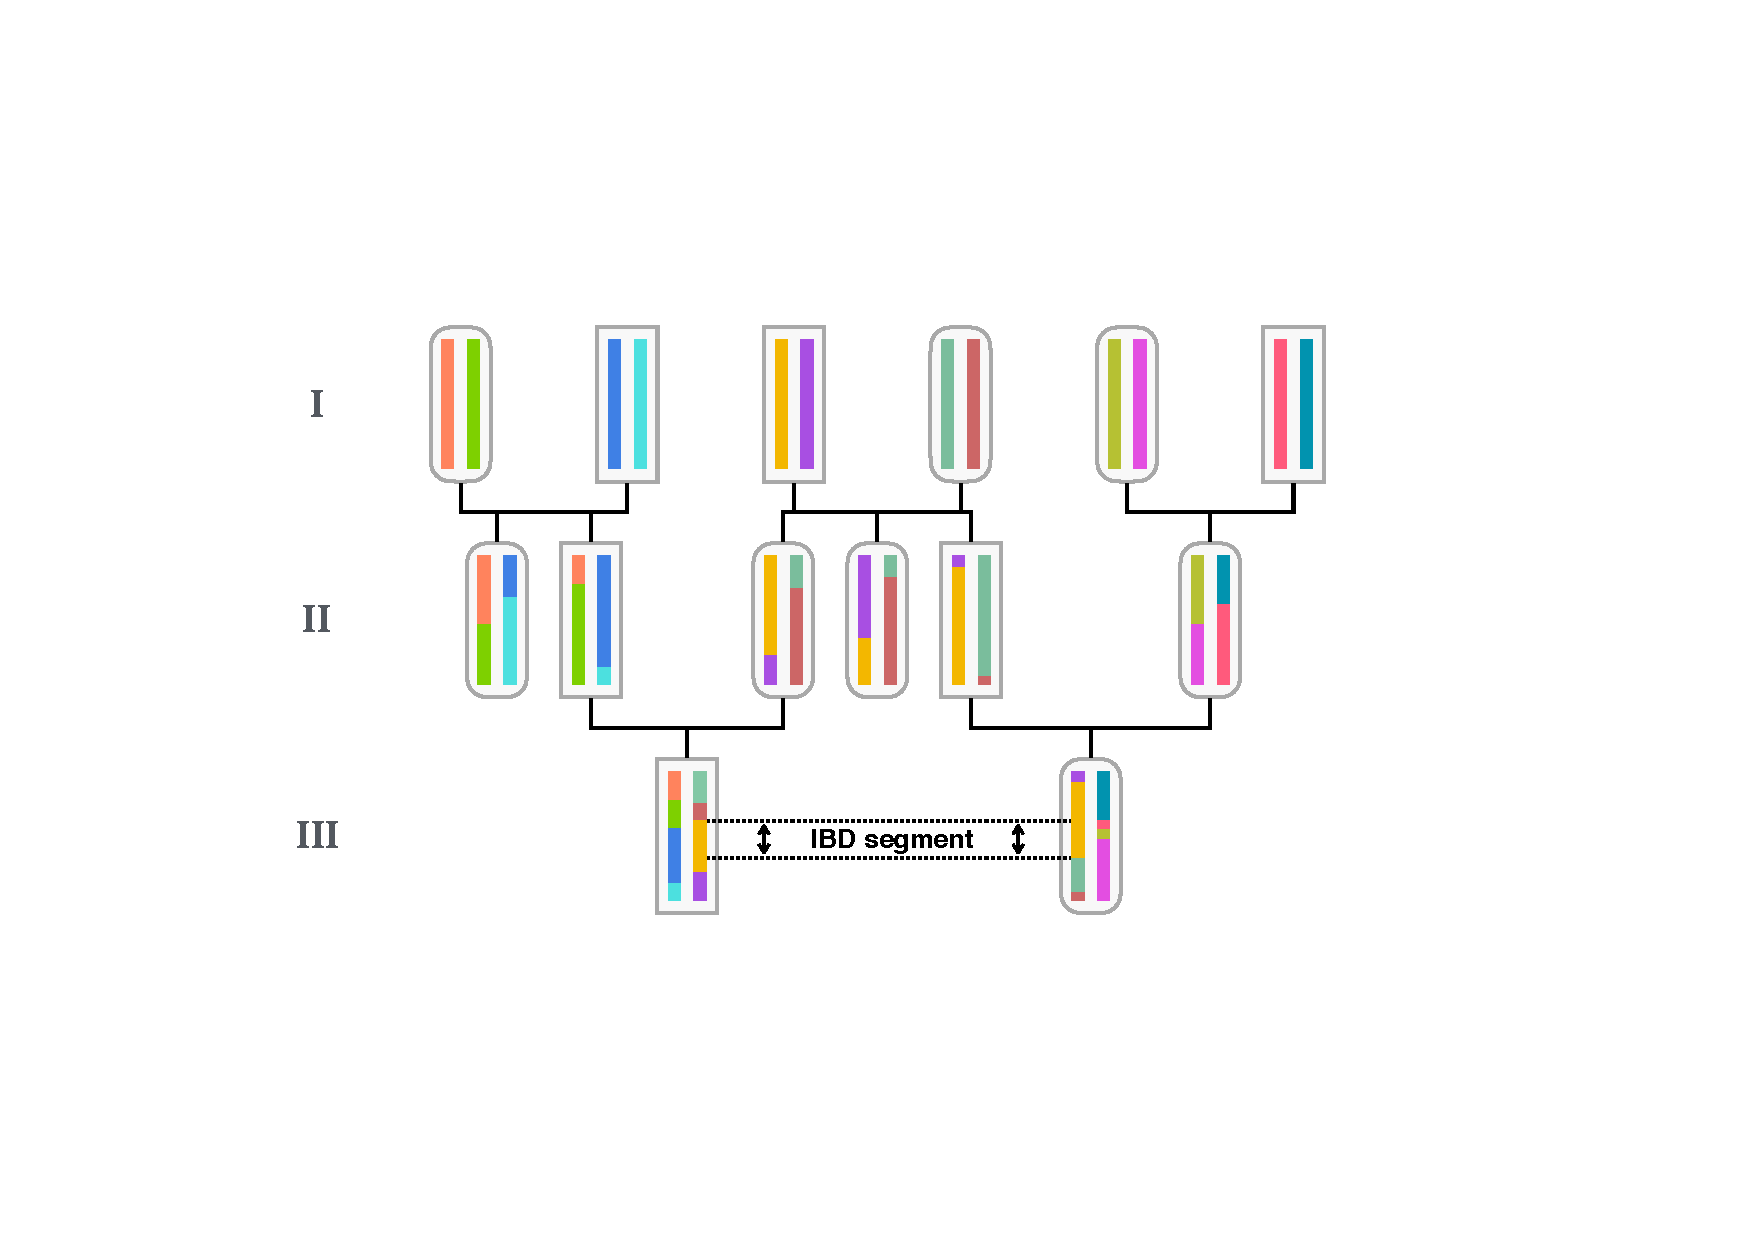
\includegraphics[width=\textwidth]{./img/ch1/info_ibd}
{\small\texthv{\textbf{(b)}}} \\
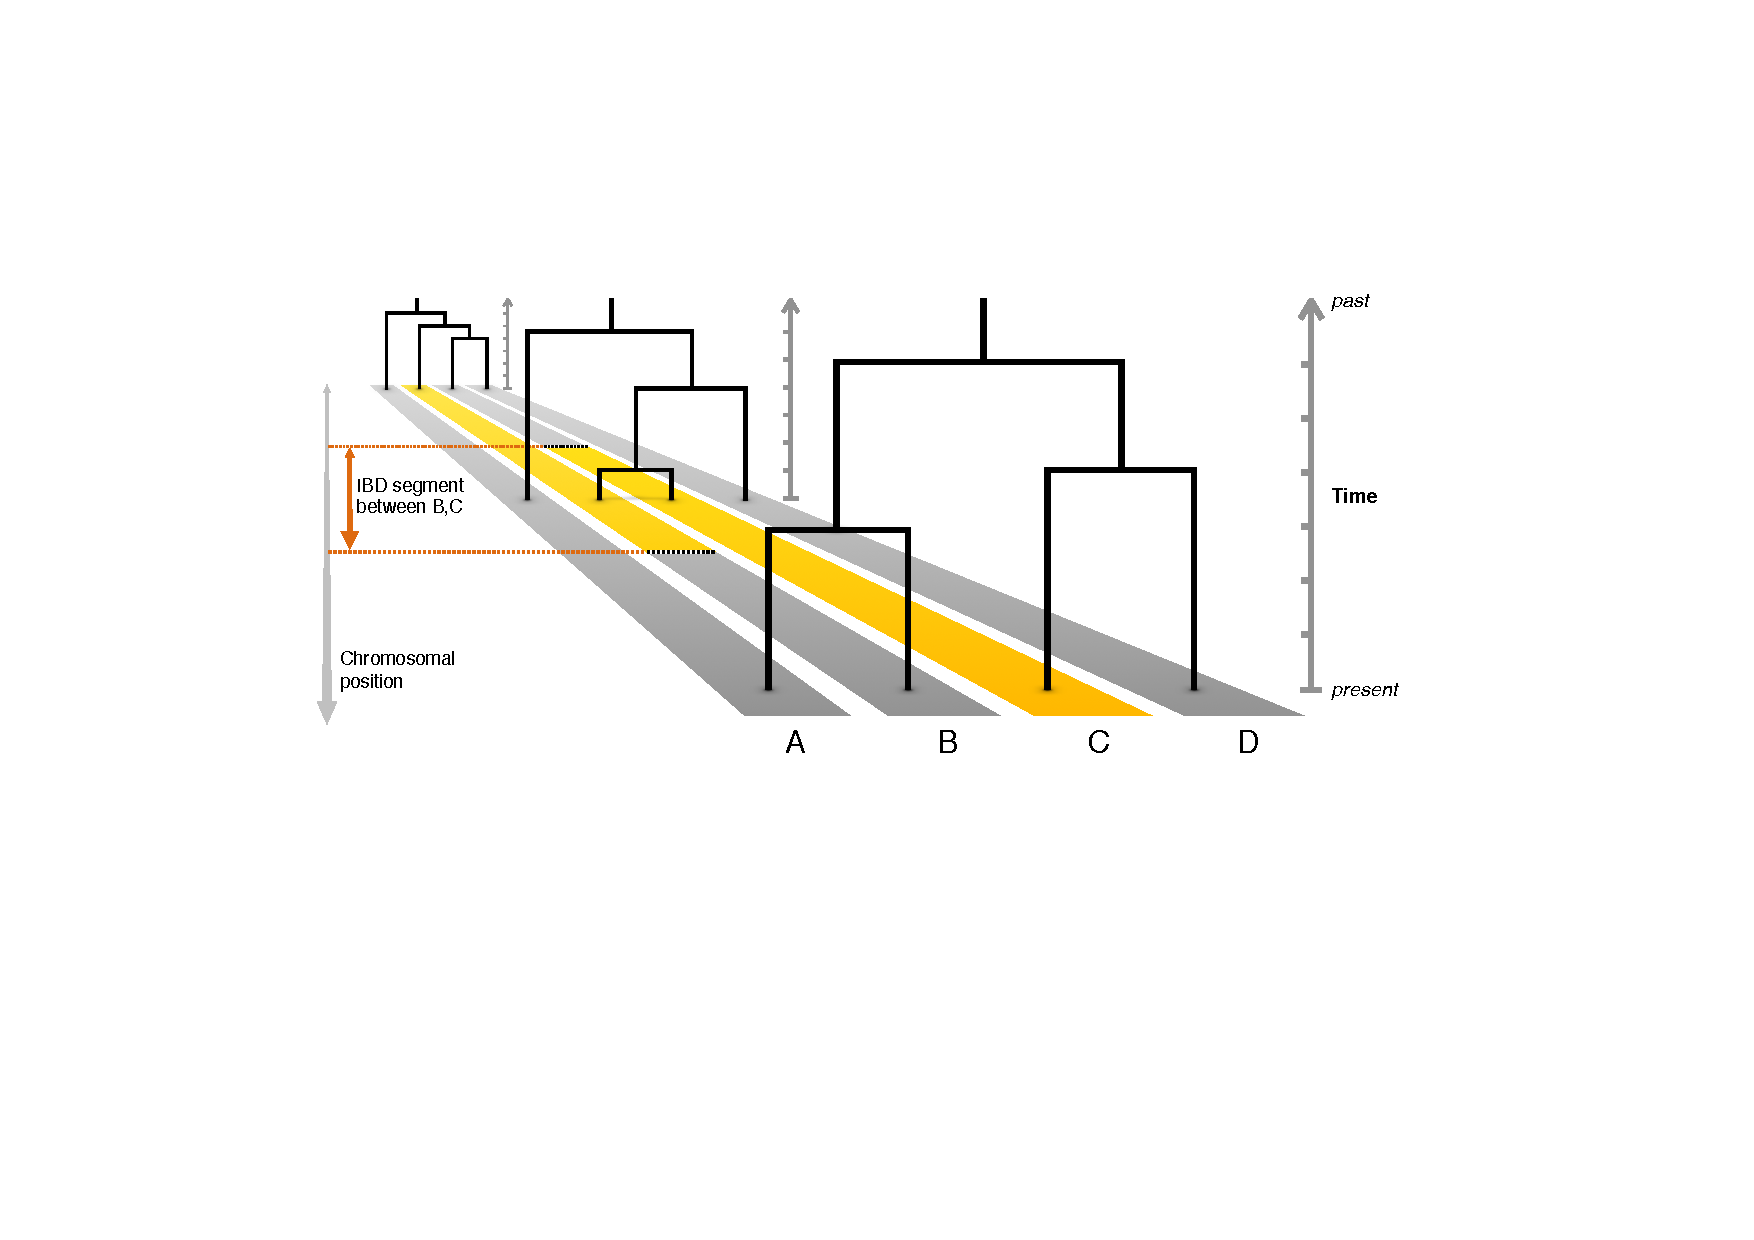
\includegraphics[width=\textwidth]{./img/ch1/info_ibd_segment}
\Caption{Illustration of haplotype sharing by descent}
{Panel~\textbf{(a)} shows a \n{3}-generation pedigree; generation~\rom{1} consists of the founders of the pedigree.
The \n{2} individuals shown in generation~\rom{3} are first-degree cousins.
Male and female individuals are distinguished by square and round shapes, respectively.
Each individual carries a diploid genome, shown as \n{2} large homologous chromosomes.
The colour of each chromosome indicates the ``identity'' of the shared ancestral haplotype, which is shuffled with the other haplotype present in the same individual due to meiotic recombination in each generation, such that the offspring receives a unique arrangement of haplotype segments per chromosome from each parent.
The ``shared'' haplotype refers the the overlapping region of haplotypes that are identical by descent; \ie the IBD segment shared by the \n{2} individuals in generation~\rom{3}, indicated by the \emph{orange} ancestral haplotype.
For simplicity, all founders are shown with the same colour.
Panel~\textbf{(b)} illustrates the different genealogies along the length of the sequence of \n{4} chromosomes (A, B, C, and D), indicated by \n{3} marginal trees.
The IBD segment co-inherited by chromosomes B and C is found at the overlapping region of the shared ancestral haplotype of the \gls{mrca} (\emph{orange}).
Note that the \n{4} chromosomes given in Panel~(b) show a simpler arrangement of haplotypes than shown in Panel~(a).}
{fig:info_ibd}
\end{figure}

%

% The concept of \gls{ibd} is illustrated by a simple example in \cpref{fig:info_ibd}.



% The transmission of genetic material from the parents to their offspring
% implies that
% is a copy of
%
% % A pedigree is a group of individuals together with a full specification of all the
% % relationships between them (Thompson, 1986). Individuals without parents in the pedigree
% % are founders, are unrelated by definition, and can either be recent or belong to some
% % baseline ancestral generation of interest. Pedigree members with mutual offspring in the
% % pedigree are spouses and every spouse pairing is a marriage.
%
% The concept of \gls{ibd} was first articulated by
%
% \citet{cotterman1940calculus}
% \citet{malecot1948mathematics}
%
%
%

% IBD is broken down through recombination in the formation of gametes during meiosis
% reduction of IBD length over generations
%



%
% \section{Genetic background of disease}
%


%\citep{Mendel1866}


% One of the primary aims of genetic research is to find connections between phenotype and genotype.
%
%
% genetic interaction
% age of disease onset
%
% unambiguous diagnosis of a disease trait
% one-to-one correspondence between a trait and a mutation directly causing its expression.
%
% phenotypes controlled by a single gene
% the result of mutations at a single gene locus
%
% patterns of Mendelian inheritance
%
% Since such phenotypes typically segregate within families, classic linkage analysis considers pedigree information to
%
% Phenotypes
% also referred to as Mendelian traits or disorders
%
% highly penetrant




%
% %!TEX root = ../../main.tex


\begin{figure}[!htb]
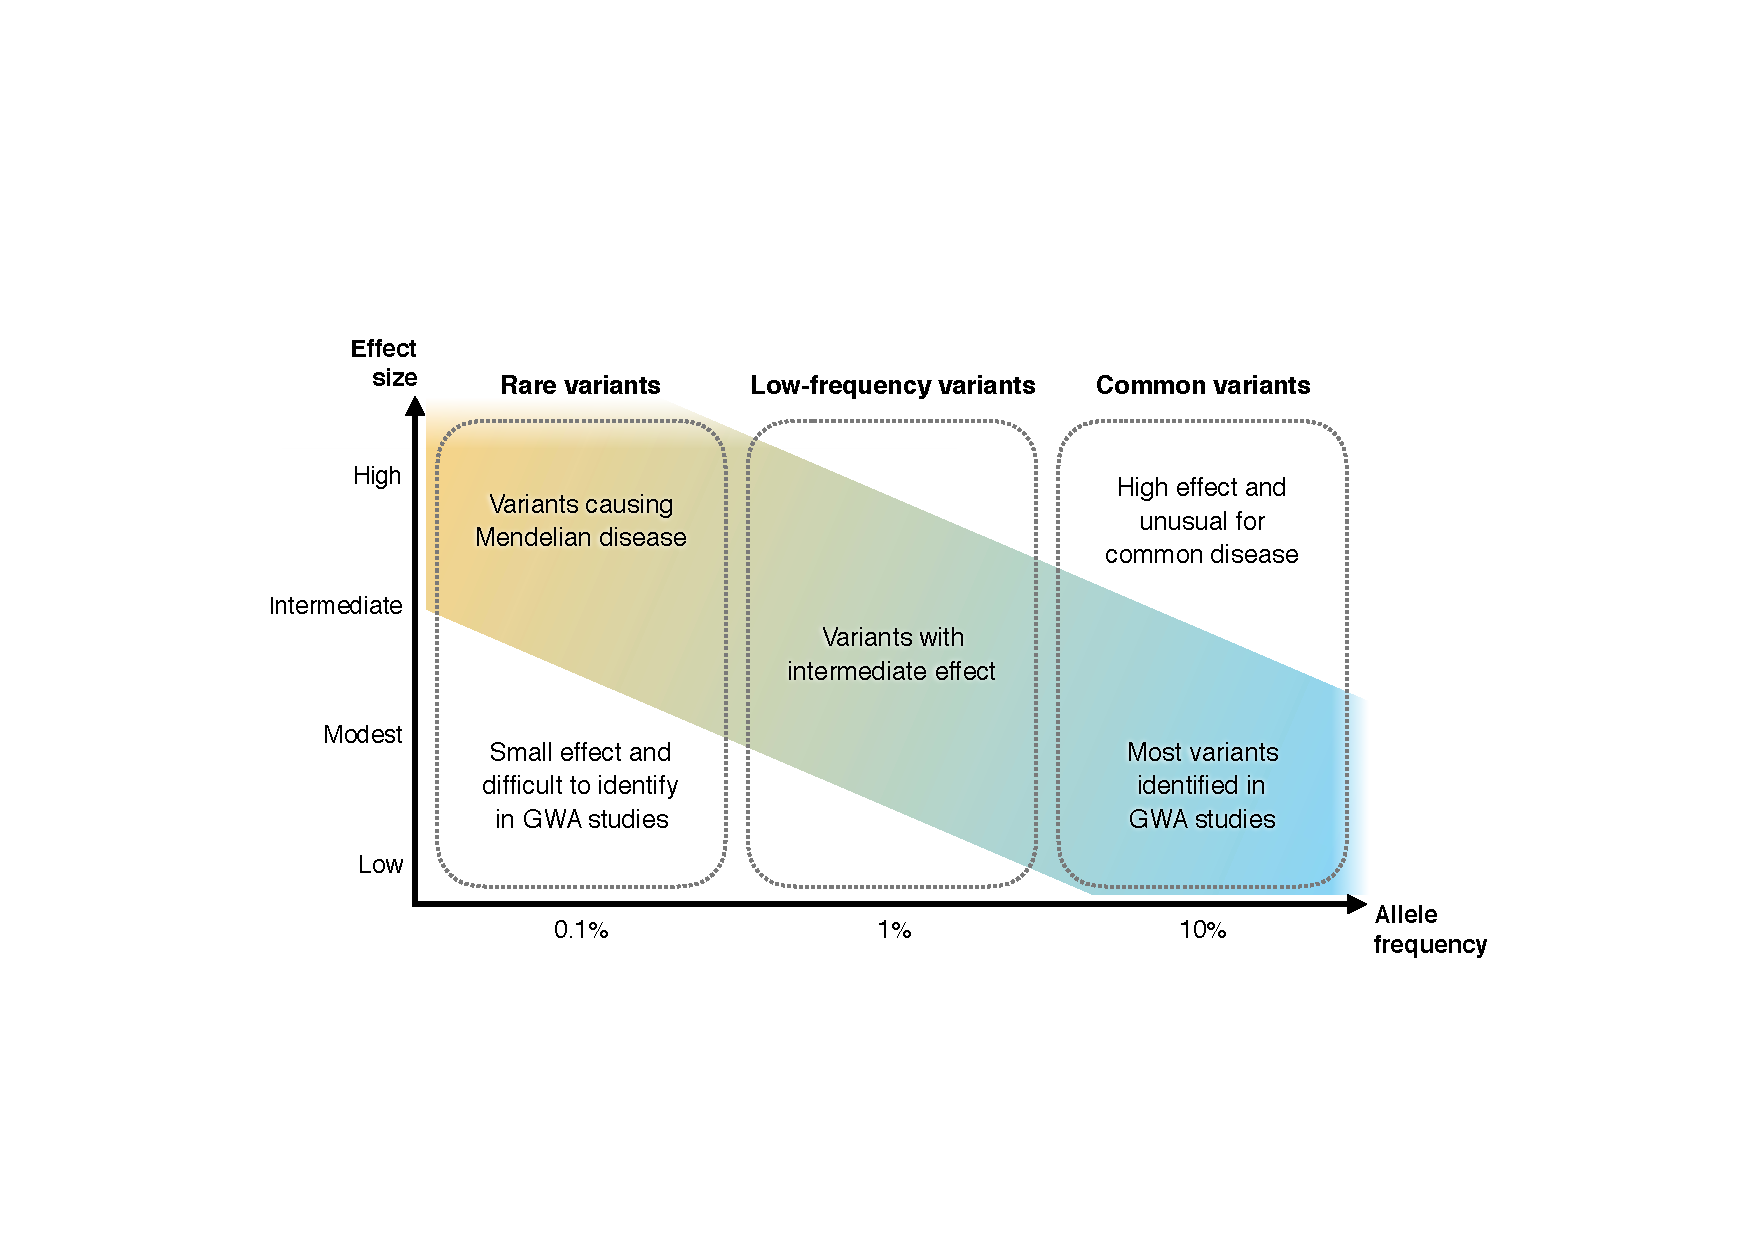
\includegraphics[width=\textwidth]{./img/ch1/gwa_spectrum}
\Caption{Risk-related variants by allele frequency and effect size}
{Rare, low-frequency, and common variants are distinguished by (minor) allele frequency.
Note that frequency values are only indicated as approximate guides.
Figure adapted from \citet[][Box~7]{McCarthy:2008il} and \citet[][Figure~1]{Manolio:2009jp}.}
{fig:gwa_spectrum}
\end{figure}

%




%
% \subsection{Linkage analysis of Mendelian disease}
%

% the rate of recombination along a chromosome is a measure of genetic linkage
%
% One of the first successes accomplished by linkage analysis was the identification of the cystic fibrosis gene \citep{Kerem:1989uz}.
%
%
% known mendelian disorders
% a catalog of mendelian traits and disorders


%
% \subsection{Genome-wide association analysis of complex disease}
%









% To date, more than \n{2700} studies have contributed to the NHGRI-EBI Catalogue of publicly available \gls{gwa} results \citep{Welter:2014dj}, where more than \n{30000} unique disease risk associations are documented\footnote{NHGRI-EBI Catalogue: \url{http://www.ebi.ac.uk/gwas/} \accessed{2017}{01}{20}}.
%
%  have been identified to be significantly associated (p-value~$\leq\num{5e-8}$) to one or several complex traits .
%
% the majority of identified variants (\dec{0.8706842}\%) was above \gls{maf}~10\%.
% Likewise, \dec{0.8323917}\% of variants was reported with an \gls{or} below~2.

%
% %!TEX root = ../../main.tex


\begin{figure}[!htb]
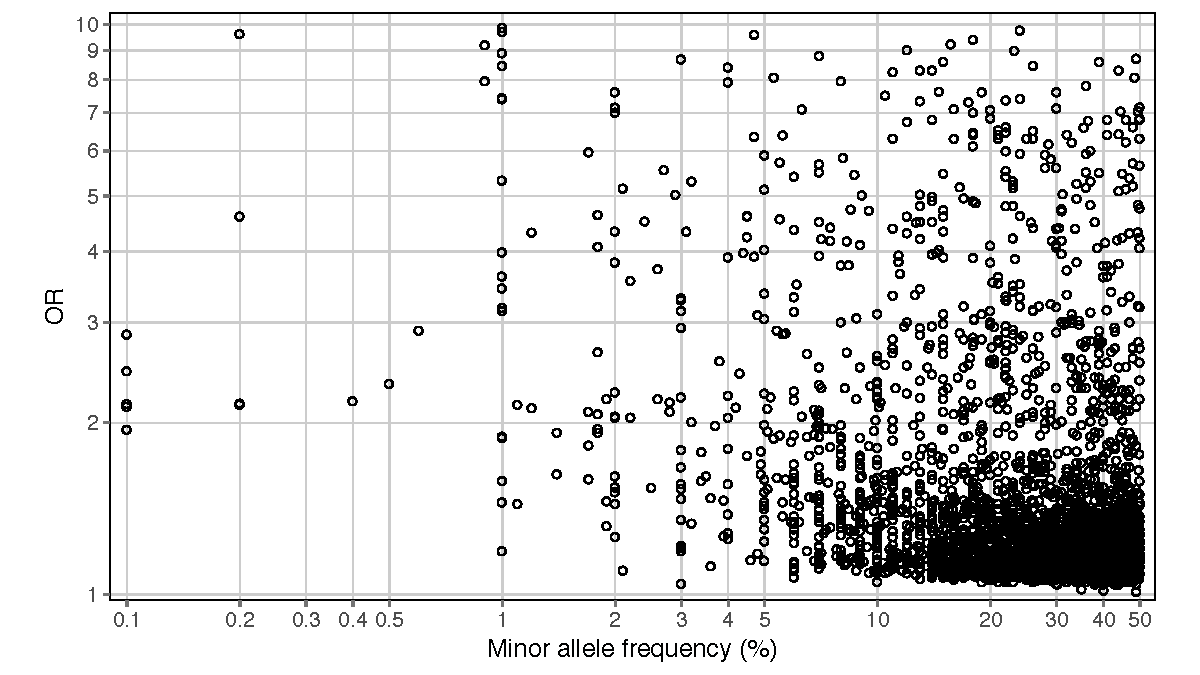
\includegraphics[width=\textwidth]{./img/ch1/gwascat}
\Caption{Significant risk-associated variants listed in the NHGRI-EBI Catalogue}
{Results are shown for \n{3186}~unique variants which were reported as being significant at ${\pvalue\leq\num{5e-8}}$ and for which \gls{or} values were available in the database.
Note that different studies may report different \gls{maf} and \gls{or}.
Duplicate entries (variants reported in more than \n{1} study) were removed, after calculating the median value of \gls{maf} and \gls{or} across duplicates; frequencies were then rounded to \n{3} decimal places.
Data were taken from \url{http://www.ebi.ac.uk/gwas/} \accessed{2017}{01}{20}.}
{fig:gwascat}
\end{figure}

%

% \cpref{fig:gwa_spectrum}


%
\section{Genetic datasets}
%

-- technology (genotyping vs sequencing), NGS
-- advancements, growth of datasets, Moore's Law
-- the Human Genome Project
-- relevant datasets used in this thesis: HapMap, 1000G, UK Biobank
-- ethics regulations
-- data formats
-- computational challenges


%
\section{Aims and structure of this thesis}
%


The main goal of this thesis is the development of novel statistical methods for the analysis of rare and low-frequency variants.
This section provides an introduction to the following \n{2}~questions, after which the objectives of this thesis are outlined as addressed in each chapter.

so as to better understand their role in the aetiology of complex disease.
Primarily, however, this thesis intends to develop the toolset necessary to extract information from rare variants directly

%%% implications of rare variants:
For more than a decade we have hypothesized that rare variants contribute to disease susceptibility \citep{Pritchard:2001hw}.
Although a given allele may be shared by less than 5\% of individuals in the population, its importance may be inversely proportional to its frequency \citep{Manolio:2009jp}.
However, we still lack sufficient means to better understand how rare variants are implicated in the genetic architecture of complex traits, and how they influence fitness and risk for certain diseases.

In general, low-frequency variants tend to be population-specific, but also highly differentiated between demographic groups on a finer scale \citep{Gravel:2011bg,Bustamante:2011df,Mathieson:2014ig}.
This is because rare variants are likely to have a relatively recent origin through mutation; i.e., they are "young" in age.
Conversely, genetic factors that contribute to substantial disease risk (particularly with early onset) are likely to be under purifying selection, which implies that they should be observed at relatively low frequencies \citep{Pritchard:2001hw,Kryukov:2007ec,Marth:2011bz}.

%%% Rare variants problem:
-- most variant sites are rare, ie. the allele at a given site in the genome is shared by only a few individuals in the population
-- given their low frequency, it is difficult to capture variants that occur at very low frequencies
-- because they may segregate only within families, isolated sub-populations
-- technological limits: genotyping chips/arrays not designed to capture low-frequency variants; sequencing may
-- in \gls{gwa}, rare variants are generally expected to be too low in frequency to expect significant associations to traits

rare variants are highly population-specific
too rare to expect statistical significance, for example, in GWAS where case and control cohorts are compared


The objective of the first chapter, following this introduction, concerns the availability of data and the resulting limitations to the interrogation of low-frequency and rare variants in \gls{gwa} studies.
The following outlines the context of the problem that is addressed in Chapter~2.
To make large-scale investigation of (disease) traits feasible, \gls{gwa} studies typically use genotyping chips or arrays to generate a scaffold of sample genotypes, which capture the variation observed at a modest subset of sites in the genome.
The gaps in the scaffold are filled through statistical \emph{imputation} of variant genotypes, using the information available in a larger panel of reference haplotypes.
Consequentially, the amount of variation observed in the reference panel constitutes a limiting factor for the analysis of alleles that differ in frequency within the study cohort.
In particular, alleles observed at lower frequencies are more likely to be specific to the cohort or population being investigated, but which may be underrepresented or absent in available reference data.
Genotyping methods are typically not designed to capture genotypes at lower frequencies, which further decreases the chance to retain rare variants in \gls{gwa} data, and conversely increases the reliance on imputation from a reference panel.
Although the number of available reference datasets is constantly growing, also both in sample size and coverage, each panel by itself represents only a snapshot of the existing genetic variation in the human genome.
This ``fragmentation'' of data is addressed in Chapter~2.
A method is proposed which attempts to integrate genotype data resulting from separate imputations into a given study sample from multiple, independent reference panels.
The result is a single genotype dataset which contains the combined set of variants present across reference panels.
Thus, a larger number of variants is available for subsequent association analyses, which may also include a larger number of rare variants.
Chapter~2 describes the proposed method and evaluates whether statistical power can be improved, in particular with regard to causal risk alleles that are found at lower frequencies.



The method capitalises on the presumed young age of rare variants which makes them informative for the identification of recently inherited
-- problem: relatedness among samples causes a bias in analyses



-- identification of relatedness, in a sample of seemingly unrelated individuals
-- inference of recombination events and segments of shared ancestry; \ie \gls{ibd}
-- broad application of IBD information in genetic analyses
-- exploring the viability of a local phasing approach
-- evaluation using simulations
-- application to 1000G data


The chapters thereafter approach rare genetic variants from a different perspective.

 a different paradigm was explored.

Namely, the remaining chapters advocate a \emph{variant-centric} view
for which I developed a set of novel strategies as solutions to particular problems in statistical genetics.

in which rare variants are used as a source of information to instruct a set of novel strategies developed within this thesis.

The methods developed attempt to provide solutions to particular problems in statistical genetics.




A non-probabilistic method for targeted IBD detection is proposed in Chapter~3.

due to their presumed recent origin through mutation
rare variants are used as indicators of relatedness
identify haplotype sharing

Chapter~3 also explores to what extent IBD information obtained from rare variant sharing can support the inference of the shared haplotype sequence for the purpose of genotype phasing.
Existing phasing methods have a high accuracy, however, they typically do poorly when it comes to rare variants



What makes rare variants
\ie that an allele is rarely observed in a population


detection of IBD segments around


namely the
to encounter genotype error
where rare variants are either falsely called or typed, as well as missed or filtered entirely
In fact, many studies exclude variants if observed below a nominal allele frequency threshold (\eg <~1\%)
To address the unavoidable presence of error in real data, Chapter~4
is composed of \n{2} parts.
First, erroneous genotypes are identified in real datasets (using both sequencing and genotyping data) by comparison to a reference dataset composed of presumed ``true'' genotypes obtained on an identical set of individuals.
The results from this analysis were used to construct an empirical model of genotype error.
Second, a \gls{hmm} for inference of recombination was
which allowed to model IBD in a probabilistic

The emphasis on targeted IBD detection, which should be blatantly conspicuous by now, is explained by its central role in the theory presented in Chapter~5.
A novel method for the estimation of allelic age was developed, \ie the time since a mutation gave rise to any particular (rare) allele of interest (introducing the \emph{age} of age estimation in genomic research if so inclined).
The method
referred to as \emph{rvage} (short for rare variant age estimation)
 is based on properties of the coalescent
using information derived from mutational variation along IBD segments as well as their length
and requires


%

Whether this shall turn out to make an impact, or whether that station will be held by future research, the following chapters will show.



%%%%%%%%%%%%%%%%%%%%%%%%

Genetic and environmental factors are key forces in shaping an individual’s predisposition to disease.
Ultimately the hope is that we will be able to translate insights from the genetic makeup of diseases to therapies and cures. In the past two decades significant strides have been made in understanding the genetic makeup of complex traits.

More recently, “genome-wide association mapping” in populations has been the preferred approach. This approach consists of obtaining genotype data from over half a million markers across the genome and contrasting the frequencies observed in cases to the frequencies observed in controls from the same population. These genome-wide association studies (GWAS) of common diseases have yielded over 4,000 bona-fide associations in the genome.
In spite of that, the therapeutic promise has not yet been met. Possible contributions for this include: i) common variant associations only explain a small proportion of the disease heritability, ii) common variant associations do not yield the causal variant much less the gene by which it exerts its effect on to lead to disease predisposition, iii) associated common variants only have a small effect on disease predisposition thereby limiting the translational inferences that can be made, and iv) the main reason that GWAS is only seven years old.

In the past few years the field has gravitated towards association studies of rare variants which yields many opportunities in genetic mapping of human diseases, but produces additional challenges that were not present in earlier association mapping approaches. Most notably is the limitation to perform an association of a single marker to a trait due to the lack of information available from a single rare event. Thus, it is usually required to aggregate information across multiple markers (hereinafter referred to as variants) and in order to do so some prior understanding of the functional consequences of DNA sequence variants is necessary.



Genetische, evolutionäre und umweltbedingte Faktoren sind die Schlüsselkräfte, die bei der Ausprägung der individuellen Veranlagung von genetisch bedingten Krankheiten eine Rolle spielen.

Letztlich ist die Hoffnung, dass wir in der Lage sind, Einsichten aus dem genetischen Architectur von Krankheiten zu Therapien und Heilungen zu übersetzen. In den vergangenen zwei Jahrzehnten wurden bedeutende Fortschritte gemacht, um das genetische Make-up komplexer Merkmale zu verstehen.

In jüngster Zeit ist "genomweites Assoziations-Mapping" in Populationen der bevorzugte Ansatz. Dieser Ansatz besteht darin, Genotyp-Daten von über einer halben Million Marker über das Genom zu erhalten und die Frequenzen, die in Fällen beobachtet wurden, mit den Frequenzen zu beobachten, die bei Kontrollen von der gleichen Population beobachtet wurden. Diese genomweiten Assoziationsstudien (GWAS) von gemeinsamen Krankheiten haben über 4.000 bona-fide Assoziationen im Genom ergeben.
Trotzdem ist das therapeutische Versprechen noch nicht erfüllt. Mögliche Beiträge dazu sind: i) gemeinsame Variantenverbände erklären nur einen kleinen Teil der Erbgut der Erkrankung, ii) gemeinsame Variantenverbände geben der Kausalvariante nicht viel weniger das Gen an, mit dem sie ihre Wirkung auf die Krankheitsveranlagung ausübt, iii ) Assoziierte gemeinsame Varianten haben nur eine geringe Wirkung auf die Krankheitsveranlagung, wodurch die translatorischen Schlussfolgerungen eingeschränkt werden können, und iv) der Hauptgrund dafür, dass GWAS nur sieben Jahre alt ist.

In den vergangenen Jahren hat sich das Feld auf Assoziationsstudien seltener Varianten ausgewirkt, die viele Chancen in der genetischen Kartierung von menschlichen Krankheiten ergeben, aber zusätzliche Herausforderungen hervorbringen, die in früheren Assoziationsabbildungsansätzen nicht vorhanden waren. Es ist vor allem die Beschränkung, eine Assoziation eines einzelnen Markers zu einem Merkmal durch den Mangel an Informationen aus einem einzigen seltenen Ereignis zu führen. Somit ist es üblicherweise erforderlich, Informationen über mehrere Marker (nachfolgend als Varianten bezeichnet) zu aggregieren, und um dies zu tun, ist ein vorheriges Verständnis der funktionellen Konsequenzen von DNA-Sequenzvarianten erforderlich.





%%%%%%%%%%%%%%%%%%%%%%%%%%%%%%%%%%%%%%%%%%




% Despite the great improvements in \gls{ngs} cost efficiency, the technical capacity to store, manage, and analyse genomic data has been overtaken by the unprecedented rate of data generation.
% For example, the data stored at the \gls{ebi} currently doubles in size within less than a year \citep{Marx:2013dz}.
% Never before had the consideration of computational tractability been more important to the development of novel analytical methods.
%
% -- follow development of the computer industry
% -- cluster and cloud-based computing
% -- processor technologies; parallelisation on multi-core systems and vectorisation of computation
% -- programming languages
%
% For example, the computational methods that I developed in this work were prototyped using high-level (simple but slow) languages such as \texttt{R} or \texttt{python}, but which I eventually implemented in low-level (fast) machine code using languages such as \texthv{\smaller C} or \cpp for large-scale application and eventual generation of results.





From the formulation of the laws of genetic inheritance by \citet{Mendel1866}, their rediscovery some decades later \citep{correns1899,vries1900,tschermak1900}, until after the completion of the Human Genome Project a century later \citep{IntHumGenSeqCon:2001hk,IntHumGenSeqCon:2004bm},
only little was known about the genetic architecture of complex disease or risk-related disease traits.


Our understanding of genetic information and the forces that shape genetic variation in a population has grown since the early breeding experiments on pea plants conducted by \citet{Mendel1866}, who formulated the fundamental laws of inheritance, which were then rediscovery more than \n{30}~years later \citep{correns1899,vries1900,tschermak1900}.
One of the main goals of modern genetic research is to learn about the genetic architecture that underpins heritable disease traits.
The early efforts in disease research were directed towards the identification of genetic variants with highly penetrant effects on disease risk; \eg mutations that contribute to a distinct phenotype such as cystic fibrosis or Huntington’s disease, which tend to segregate within families (\ie \emph{monogenic} or \emph{Mendelian} diseases).

The classical approach to locate (or ``map'') the genetic factors involved in such ``simple'' diseases is linkage mapping within affected families \citep[\eg, see][]{morris2007}.
While linkage studies have been successful in the identification of genetic factors underlying Mendelian diseases \citep{Altshuler:2008kp}, they have been less successful with regard to locating variants that influence complex diseases, such as type~2 diabetes, as each variant by itself may only contribute modestly to disease susceptibility \citep{Risch:2000jb,Botstein:2003kf}.
-- More recently, GWAS have been the preferred method; to interrogate common variants;
-- are more powerful for the analysis of complex traits.
-- Much of what we now know about the human genome as well as the genetic architecture underlying complex disease has been gained in the past decade, due to the advances made in the human genome project, HapMap, 1000G etc.
-- GWAS have been a driving force in this development and has uncovered significant associations between thousands of genetic factors and major common diseases
-- However, an emerging view is that rare variants could be involved [have an important role/are more important than previously thought] in the predisposition to complex disease {Ott:2015il}.

One major insight gained from the extensive study of the (human) genome is that the genetic variation between individuals is mostly determined by \emph{common} variants, referring to alleles observed at higher frequencies, \eg \gls{maf}~${\geq 5}$\%, but most variant sites in the genome are \emph{rare}.
Although a particular allele may be shared by only a small fraction of individuals in the population (thus being ``rare''), the importance of rare alleles with regard to complex disease may be inversely proportional to their frequency \citep{Bodmer:2008ep,Schork:2009ke,Manolio:2009jp,Cirulli:2010cza}.
For more than a decade, it has been hypothesised that rare variants contribute to disease susceptibility \citep{Pritchard:2001hw}.
However, the interrogation of alleles found at lower frequencies is not straightforward.
For instance, \gls{gwa} methods are designed to examine common variants, as rare variants are generally too low in frequency to expect statistical significance and are therefore underpowered in association tests.

For more than a decade we have hypothesized that rare variants contribute to disease susceptibility \citep{Pritchard:2001hw}.
Although a given allele may be shared by less than 5\% of individuals in the population, its importance may be inversely proportional to its frequency \citep{Manolio:2009jp}.
However, we still lack sufficient means to better understand how rare variants are implicated in the genetic architecture of complex traits, and how they influence fitness and risk for certain diseases.

In general, low-frequency variants tend to be population-specific, but also highly differentiated between demographic groups on a finer scale \citep{Gravel:2011bg,Bustamante:2011df,Mathieson:2014ig}.
This is because rare variants are likely to have a relatively recent origin through mutation; i.e., they are "young" in age.
Conversely, genetic factors that contribute to substantial disease risk (particularly with early onset) are likely to be under purifying selection, which implies that they should be observed at relatively low frequencies \citep{Pritchard:2001hw,Kryukov:2007ec,Marth:2011bz}.

-- most variant sites are rare, ie. the allele at a given site in the genome is shared by only a few individuals in the population
-- given their low frequency, it is difficult to capture variants that occur at very low frequencies
-- because they may segregate only within families, isolated sub-populations
-- technological limits: genotyping chips/arrays not designed to capture low-frequency variants; sequencing may
-- in \gls{gwa}, rare variants are generally expected to be too low in frequency to expect significant associations to traits




Perhaps a fitting analogy would be to compare rare variants to the accumulation of sand in the gears of an engine.
Over time, the sand particles form more heavy clumps and deposit at certain corners, which are commonly seen in engines of the same make, either due to the same forces that act on the overall machine or simply due to random drift [my idea, no ref.].


{Cooper:2010iq}



linkage studies have been much less success- ful in locating genetic variants that affect common complex dis- eases, as each variant individually contributes only modestly to disease risk
GWAS the preferential strategy to implicate risk-related factors
proven to be a powerful tool for identifying the genetic factors underlying Mendelian diseases



After the human genome has been mapped and the nucleotide sequence
little was known about the genetic architecture that underlies disease susceptibility.
It was the prevalent hypothesis that the genetic factors involved in the predisposition of complex disease should also be common in the population
\citep{Lander:1996fj,Chakravarti:1999ic}.


Any findings that may implicate rare variants should also be treated with caution, due to the technical difficulty to determine

The importance of rare alleles may be inversely proportional to their frequency.




genetic markers in close physical proximity
which is based on the observation that genetic markers that sit in close physical proximity to each other tend to segregate together following recombination over multiple generations.
Genetic markers are mapped
and can thereby be found
powerful to identify highly penetrant
correlation
within larger family pedigrees or smaller family units
successful identification of hundreds of genes contributing to
\citep{Altshuler:2008kp}.
Recently, due to the rapid advances in genotyping and \gls{ngs} technologies,

However, there are still many questions that remain and big challenges that lie ahead.

which perhaps can be described as the leading paradigm of the analytical approach to understand complex disease.

Since it became possible to map the human genome and decode the sequence of nucleotides
The field of statistical genetics has evolved from a theoretical field of study into an active and highly dynamic area of applied research.
In particular, due to recent advances in genotyping and \gls{ngs} technologies, the field has adapted to the exponential growth of available molecular data and continues to fill a niche in both the computational and mathematical sciences, so as to be able to analyse the increasing amounts of data and to answer questions of biological as well as medical meaning.




% since it became possible to decode the sequence of individual genomes
% our goal is to learn more about the genetic architecture of disease
% linkage analysis for the identification of factors involved in rare diseases
% identified hundreds of genes associated with Mendelian diseases
% less successful for common diseases

% gwas have been instrumental for common diseases
% identified thousands of genetic risk factors
% motivated the collection of very large datasets
% thereby driving the progress in genomic technologies and industry
% recent advances in genomic technologies revealed unprecedented details

% however, identified factors explain only a fraction of heritability
% most identified factors have a small effect size
% a main problem is that gwas cannot pinpoint causal variants or genes
% gwas have not delivered on the promise to result in therapeutic applications




% one major insight is that most variants are rare
% they may be important to our understanding of disease
% but the problems are:
% gwas are designed to interrogate common variants
% statistical tests are underpowered, because an allele is simply too rare
% they should be treated with caution, due to higher rates of genotype error
% nonetheless, several studies have found rare variant associations [examples]
% the signal found at a common variant may be explained by many rare variants
% thus, there is a recession of the "common disease, common variant" hypothesis


% new strategies required to learn more about the genetic architecture

% Which genetic factors are implicated in a certain disease?
% What can be learned from the genetic variants observed to elucidate disease?

% we want to learn about the processes that created observed genetic variation


Our knowledge about the genetic factors involved in the predisposition of disease has grown since the





S.~Wright, J.B.S.~Haldane, and R.A.~Fisher

Even before the discovery of the molecular structure of \gls{dna} by \citet{Watson:1953ug}, on basis of X-ray diffraction data by R.~Franklin,


Over the last century, the field of population genetics has evolved from a mainly theoretical area of study into a more applied area of research.
More recently, the field has adapted to the exponential growth of available molecular data and continues to fill a niche in the computational sciences so as to be able to analyse the increasing amounts of data and to answer questions of biological as well as medical meaning.


, such as ...
However, despite those exciting insights, there remain many challenges to be addressed and promises not yet fulfilled.

One major insight from the extensive study of the human genome has been that most of the genetic variation observed between individuals is found at common sites, \ie variants that segregate at higher frequencies in a population (\eg MAF > 5\%), but most of the genetic variants are rare.

the completion of the sequence of the human genome \citep{InternationalHumanGenomeSequencingConsortium:2001hk,Venter:2001fq,InternationalHumanGenomeSequencingConsortium:2004bm}
and large-scale studies such as the \gls{hapmap}, the \gls{1kg}, the \gls{uk10k}, and the UK~Biobank

There is now an abundance of data
hundreds of thousands of individual genomes have been assessed

In this work,


In particular, rare variants are utilised as a source of information about recent relatedness among the individuals in a sample, which follows from their presumed recent origin through mutation.

In the last section of this chapter, I provide a brief summary of the problems and objectives addressed in each chapter, as a reminder of what I outlined in the section above.









% the information contained in the human genome entails the history of the population
% by learning about it, we can also learn more about the genetic architecture of disease
% it is the hope that this knowledge can be translated into therapeutic applications
% we want to learn about the processes that created observed genetic variation
% progress made in human genetics
% genome-wide sequencing has enabled insights into the human genome on an unprecedented sale [examples for large-scale studies]
% gwas instrumental in discovery/identification of thousands of genetic factors
% gwas design partly motivated by common-disease-common-variant hypothesis
% association analyses are innately underpowered when it comes to the interrogation of rare and low-frequency variants
% many insights, but also many big challenges

% one insight (and challenge) is given by rare variants
% in gwas, rare variants are too low in frequency to expect significant findings
% however, many rare factors have been implicated [examples?]
% more so, over a decade, rare variants have been suspected to play a role
% for example, alleles under purifying selection should be low in frequency
% however, there is much to learn from rare variants
% properties: presumed young age, specific occurrence in populations
% indicators of recent relatedness, thereby useful to identify long stretches of shared ancestry (shared haplotypes, IBD)

% ever since the experiments conducted by Mendel, from which the Mendelian laws of inheritance derive, our understanding of genetic variation and the processes that generate it has grown, due to the theoretical works pioneered by [names]




Over the last century, our understanding of the key forces shaping the genetic variation observable in a population




advances in
genotyping and \gls{ngs} technologies
high-throughput methods
understanding of the genetic architecture of diseases

\Gls{gwa} studies of common diseases have been instrumental in the identification of thousands of genetic risk factors
 disease aetiology.

However, many big challenges remain.





\gls{ibd}


The overall aim of this thesis is to develop and evaluate methods  to make use of the information represented by rare variants. These include improved imputation of low frequency variants for association analyses, discovery of identity by descent tracts, and allele age estimation.


In this thesis, I address the ``heads and tails'' of rare variants

There is much that can be learned from
rare variant sharing
relatedness



[...]

The following section outlines the biological concepts relevant to define basic terminology as used in this thesis.
In the sections thereafter, I introduce the guiding principles in the fields of medical and population genetics, so as to facilitate a better understanding of the motivation behind this work.
Lastly, I present each of the following chapters individually to bring the problems addressed therein into context with the objectives of this thesis.

%
% Due to the ongoing progress of research in the field of human genetics,
% The advances made in the field of human genetics have led to the discovery of thousands of genetic factors which either cause the manifestation of diseases or which are implicated in the development
% has been successful in the identification of many genetics factors that play a role
% The field of human genetics is currently advancing on an unprecedented scale, there is still
% and its core mission is to learn more about the genetic architecture of diseases and to translate this knowledge into therapeutic applications.
%
% Genetic, evolutionary and environmental factors are the key forces that play a role in the individual assessment of genetic diseases.
%



%
% The field of human genetics is advancing on an unprecedented scale.
% -- many insights have been gained
% -- more challenges have been highlighted
% -- Never has the link between population genetics and medical genetics been stronger.
%

% --
%
%
% Genetic variants that are low in frequency or rare
%
% For more than a decade we have hypothesised that rare variants contribute to disease susceptibility \citep{Pritchard:2001hw}.
% Although a given allele may be shared by only a small fraction of individuals in the population, its
% Their importance to the
%
% may be inversely proportional to their frequency \citep{Manolio:2009jp}.
%
%
% To make large-scale investigation of (disease) traits feasible, \gls{gwa} studies typically use genotyping chips or arrays to generate a scaffold of sample genotypes, which capture the variation observed at a modest subset of sites in the genome.
% The gaps in the scaffold are filled through statistical \emph{imputation} of variant genotypes, using the information available in a larger panel of reference haplotypes.
% Consequentially, the amount of variation observed in the reference panel constitutes a limiting factor for the analysis of alleles that differ in frequency within the study cohort.
% In particular, alleles observed at lower frequencies are more likely to be specific to the cohort or population being investigated, but which may be underrepresented or absent in available reference data.
%
%
% The detection of ``hidden'' relatedness in a sample of reportedly unrelated individuals is of particular interest to the
% \gls{gwa}~studies
% If not accounted for in the model
% the presence of systematic differences in the ancestry of cases and controls
% population structure
% missed or false positive association signals \citep{Freedman:2004dk,Marchini:2004cf,Price:2006cd}
%
%
% Two sides of the rare variant problem coin:
%
% The first part of this thesis
% the extension of existing methods eg gwas to work with rare variants
%
% and use of the information coming uniquely from rare variants
%




%IBD between two individuals have been classically quantified (Male ́cot 1948) following Wright’s inbreeding coefficient (Wright 1921), which prescribes probabilities of these individuals sharing two, one, or zero alleles by descent, averaged across the genome.
%\citep{Wright:1921tk}




seeks to catalyse
so as to increase the chance that significant associations can be found

Ultimately, the work presented in this thesis has the following contributions in mind.

Knowledge of allele age is of particular interest to a wide range of problems studied in both population and medical genetics.


allows to unravel the patterns of descent by observing demographic changes over time.

as it allows to ``turn back time'' and learn more about
past events and evolutionary processes which
did come into effect somewhere along the branches of a genealogical tree.

the study of population dynamics and ancestral reconstruction





In the following paragraphs, I provide a brief background to the specific problems and the objectives addressed in each chapter following this introduction.


In Chapter~2, I address the availability of haplotype reference data for imputation as a limiting factor to the interrogation of low-frequency and rare variants in \gls{gwa} studies.
On the premise that \gls{gwa} studies typically rely on imputation from a reference panel to fill the gaps in a study sample with  at lower frequencies
I present a new method

problem that \gls{gwa} studies are typically underpowered with regard to the interrogation of low-frequency and rare variants.

In particular, I propose a novel method that attempts to integrate the information available across different reference panels by combining genotype data resulting from separate imputations into a given study sample.
under the premise that this limitation arises from the reliance on imputation from available reference data.


 which is why much of this thesis is concerned with the development of an efficient and robust method for IBD detection (see Chapters~3 and 4).


\paragraph{Chapter~2} is concerned with the availability of data as a limiting factor to the interrogation of low-frequency and rare variants in \gls{gwa} studies.
Genotyping methods are typically designed to probe genetic markers that are expected to maximise the genetic variation observed between individuals, but the capacity to capture rare variants is thereby reduced.
Consequently, \gls{gwa} studies rely on imputation from a reference panel to fill the gaps with variants at lower frequencies.
In particular, alleles observed at lower frequencies are more likely to be specific to the cohort or population being investigated, but these may be underrepresented or absent in reference data.
Although available reference datasets are constantly growing in number, sample size, and coverage, each panel by itself represents only a snapshot of the existing genetic variation in the human genome.
This ``fragmentation'' of data is addressed in Chapter~2.

A method is presented which attempts to integrate the information available across different reference panels.
Notably, I propose a solution different to the one achieved by the \gls{hrc} which combined data from multiple, independently conducted studies to form a single, canonical reference for imputation \citep{McCarthy:2016gs}.
In the approach presented, genotype data are integrated after performing separate imputations from different reference panels into a given study sample.
The result is a single genotype dataset which contains the combined set of variants present across references.
Thus, a larger number of variants is available for subsequent interrogation in  association analysis, which may also include a larger number of variants at lower frequencies.

In the chapter, I describe several strategies by which imputed genotype datasets can be combined; the general method is referred to as \emph{meta-imputation}.
I then evaluate each strategy with regard to whether imputed genotype accuracy can be improved.
This is done in comparison to the other strategies proposed as well as genotype data resulting from direct imputations using single reference panels.
The best performing strategy is chosen for an extended evaluation of the statistical power to detect significant signals in association analyses, which is determined in a series of simulated case-control experiments.


\paragraph{Chapter~3} capitalises on the presumed young age of rare variants to identify (recent) relatedness in samples of reportedly unrelated individuals.
Given the site of a particular allele, it is straightforward to identify the individuals sharing that allele in sample data.
If the allele is rare, it is likely that the chromosomes carrying that allele are the nearest genealogical neighbours in the sample at that position in the sequence.
The low frequency suggests that the allele was inherited from a common ancestor only a few generations ago, such that recombination had less time to break down the length of the co-inherited haplotype region.
This insight is of particular interest to the discovery of IBD tracts, which is the main focus of Chapter~3.

A novel method is presented that utilises rare variants as ``bookmarks'' to highlight the positions at which the individuals sharing a focal allele are also likely to share a relatively long haplotype that is identical by descent.
The position of a rare allele is used as a target point around which
recombination events are inferred along the sequence to both sides of the focal position, which is done in each pair of individuals sharing the target allele.
As a result, the ``breakpoints'' of recombination events delimit the smallest interval detectable from available data in which \n{2} individuals share a haplotype; \ie the underlying IBD segment is enclosed.
Notably, the method presented is non-probabilistic and relies on the observation of certain allelic or genotypic configurations to infer recombination in pairs of diploid individuals.
\N{2} rule-based approaches are implemented which allow the detection of IBD segments in either haplotype or genotype data, respectively.

In the chapter, I attempt to demonstrate the general utility of rare variants as indicators of relatedness and population structure.
I then describe the method for targeted discovery of IBD segments, highlight anticipated limitations, and evaluate its accuracy by using data obtained from coalescent simulations.
By doing so, the accuracy of detected recombination breakpoints can be measured in relation to the underlying true IBD structure of the sample (known from simulation records).
This is done to quantify differences between the haplotype and genotype-based approach, and for comparisons to a competing method for IBD discovery.
The resulting distributions of inferred segment lengths provide an expectation for the analysis of real data.
In addition, I explore the viability of using IBD information obtained from genotype data to distinguish haplotypes, \ie to locally \emph{phase} genotypes based on the inferred allelic sequence of the shared haplotype.


\paragraph{Chapter~4} examines genotype error and the effects of such (minor) inaccuracies on the inference of relatedness and IBD.
The accuracy of data produced by current genotyping or sequencing technologies is sufficiently high for general analytical purposes.
However, the presence of even minor amounts of genotype error may affect the IBD detection method described in Chapter~3 in \n{2} ways.
First, it is possible that a fraction of rare variants is irretrievably missed while some alleles are falsely observed, thereby wrongly identifying haplotype sharing at a focal position.
This is particularly problematic because error rates are typically seen to increase towards the lower end of the frequency spectrum.
In practice, many studies therefore treat rare variants with caution or even exclude sites if seen below a certain frequency threshold.
Second, because recombination breakpoints are detected by scanning the regions distal to a given target site, genotype errors at sites along the sequence may lead to the discovery of false breakpoints or the disregard of actual breakpoints.
The implications of such errors are the subject of this chapter.
Note that Chapter~4 can be seen as an extension to the evaluation conducted in Chapter~3; however, a separate consideration is warranted by the different nature of the problem and the chain of consecutive analyses conducted to arrive at a solution to the problem, which is outlined below.

In the chapter, I provide a generic model to describe the ``penetrance'' of error, from which I derive theoretical expectations for misclassification rates in genotype data.
The main goal, however, is to establish an empirical model of frequency-dependent error rates based on observed misclassifications in real data, which I establish for datasets obtained on different genotyping and sequencing platforms.
I then use this information to induce realistic proportions of genotype error in simulated data, so as to quantify the impact of genotype error on IBD detection using the same evaluation procedure as in Chapter~3 and in comparison to the results obtained before the inclusion of error.
In conclusion of this chapter, I propose a probabilistic extension to the previously presented method for the targeted detection of IBD segments.
This method is implemented as a \gls{hmm} which incorporates the generated empirical error model.
I show that the \gls{hmm}-based approach is able to achieve similar levels of accuracy compared to the previously presented non-probabilistic method if genotype error is absent, and that the same level of accuracy is maintained if genotype error is present.


\paragraph{Chapter~5} proposes a novel method for the estimation of the age of (rare) alleles, \ie the time since a mutation event gave rise to a particular allele that is observed in sample data.
While the frequency of an allele is itself an estimator for the age of that allele \citep{Kimura:1973ug,Griffiths:2013ec}, the frequency measure alone does not distinguish between differences in mutational timing of alleles that are observed at the same frequency.
Detailed knowledge about the genealogy of the sample and the demographic history of the population would be required to unravel the complex relations between the demographic processes which resulted in the observed genetic variation.
For example, genetic factors that contribute to substantial disease risk (particularly with early onset) are likely to be under purifying selection, which implies that they should be observed at relatively low frequencies \citep{Pritchard:2001hw,Kryukov:2007ec,Marth:2011bz}.
The age estimation method presented in this chapter does not require such prior knowledge, but derives information from the underlying IBD structure, which is inferred through the targeted IBD detection method presented in Chapters~3 and 4.
Conversely, by knowing the age of an allele, much can be learned about the changes that occurred over time in a population.

In the chapter, I present \n{3} approaches to estimate the time of a coalescent event that separates a pair of individuals; these are based on mutational variation, the genetic distance between recombination breakpoints, and the combination of both, respectively; the general approach is referred to as the \gls{ccf}.
An age estimate for a given target allele is derived from patterns of haplotype sharing and the inferred coalescent times using a composite likelihood approach.
I demonstrate the feasibility of this method by comparing the estimated age of an allele to its true age (known from simulation records), both before and after the inclusion of genotype error.
Lastly, I estimate the ages of alleles in real data and discuss the results with regard to the consequences of predicted variant effects.







%%%%%%%%%%%%%%%%%



The next decade is likely to see further developments in the direction of personalised medicine and an increased clinical application of genomic technologies \citep{Hamburg:2010ig}.


The advances in \gls{ngs} technologies have also made the development of high-throughput genotyping technologies possible, by which the nucleotides at thousands or millions of previously identified\gls{snp} markers are interrogated simultaneously.
The first `whole-genome' \gls{snp} genotyping array was the \emph{GeneChip~10K} by \textsl{Affymetrix} \citep{Kennedy:2003ht}.
Currently, the maximum genotyping capacity is around \n{5}~million \glspl{snp} per array using the \emph{Omni5.0 Beadchip} by \textsl{Illumina} \citep{Ragoussis:2009kb}.





%
\subsubsection{Linkage disequilibrium}
%

The linkage structure of markers across the genome is essential for fine-scale mapping of human disease loci \citep{Risch:1996ub,Cardon:2001cj}.
Allelic association at \n{2} (or multiple) markers is expressed by the (potentially misleading) term \gls{ld}, which was introduced by \citet{Lewontin:1960he} and refers to the statistically non-independent association of alleles at different loci.
Note that linkage and linkage disequilibrium are conceptually different; while genetic linkage refers to the alleles at \n{2} or more loci which are transmitted together on the same chromosome without being separated by meiotic recombination, \gls{ld} merely refers to the statistical correlation between alleles, which may arise through genetic linkage but can be influenced by differences in allele frequencies (\eg population structure).

Consider a haplotype with \n{2} loci; $\mathcal{A}$ with alleles $A$ and $a$, and $\mathcal{B}$ with $B$ and $b$.
Let $\pi$ denote the frequency of an allele in a sample of haplotypes, such that ${\pi_A = 1 - \pi_a}$ and ${\pi_B = 1 - \pi_b}$.
If the \n{2} loci are independent, the expected frequency of a given allelic configuration is equal to the product of allele frequencies; for example, the configuration $(A,B)$, \ie the $AB$~haplotype, is expected to be at frequency ${\pi_{AB} = \pi_A \pi_B}$, that is, if the occurrence of both alleles on the same haplotype is random.
The coefficient of \gls{ld} at the \n{2} loci is defined as the covariance of alleles $A$ and $B$, namely
\begin{equation}
	D_{AB}~=~\pi_{AB} - \pi_A \pi_B\ ,
\end{equation}
and likewise for the other possible configurations ($D_{Ab}$, $D_{aB}$, $D_{ab}$).
Note that it is sufficient to calculate $D$ for only \n{1} pair of alleles (if both loci are biallelic), due to the relation ${D_{AB} = -D_{Ab} = -D_{aB} = D_{ab}}$.
The \n{2} loci are said to be in \emph{linkage equilibrium} if ${D=0}$, or in \emph{linkage disequilibrium} otherwise.
Although the extent of \gls{ld} is fully characterised by the coefficient $D$, its value may not be interpreted conclusively because it is restricted by the allele frequencies at the \n{2} loci \citep{Slatkin:2008ks}.
A commonly applied statistic to measure \gls{ld} is the Pearson correlation coefficient, $r$, which is defined as the covariance divided by the product of the standard deviation of \n{2} variables.
It is convenient to measure \gls{ld} using the squared correlation coefficient,
\begin{equation}
	r^2 ~=~ \bigg( \frac{D_{AB}}{\sqrt{\pi_A \pi_a \pi_B \pi_b}} \bigg)^2 ~=~ \frac{D^2}{\pi_A \pi_a \pi_B \pi_b}\ ,
\end{equation}
due to the relation ${D^2 = D_{AB}^2 = D_{Ab}^2 = D_{aB}^2 = D_{ab}^2}$.



%Such an effort would necessarily mean to consider
% relax the conditions that were initially set to determine
% as it is expected that

% counterintuitive
% while the majority of variants observed in a population are rare, \eg see \cpref{fig:allelefreq_1kg},
% \citep{Lander:1996fj,Reich:2001ve}
% yet
% \citep{Simons:2014fj}
%
% A counterintuitive observation is that
% while the SFS suggests that the majority of rare variants in a population are rare, at
% the level of a single individual most variant alleles observed are actually from common
% variants.
%This observation has been used to argue in favor for the common variant
% common disease (CVCD) hypothesis that predicts that common disease-causing alleles
% will be found in all human populations which manifest a given disease (Lander,
% 1996; Reich and Lander, 2001).
